%-----------------------------------------------------------------------------%
\addChapter{lampiran-contoh-bank-pohon}
\chapter*{Lampiran 1: Contoh Bank Pohon Struktur Dependensi}
%-----------------------------------------------------------------------------%
%Lampiran merupakan data atau pelengkap atau hasil olahan yang menunjang penulisan tugas akhir, tetapi tidak dicantumkan di dalam isi tugas akhir, karena akan mengganggu kesinambungan pembacaan. Lampiran yang perlu disertakan dikelompokkan menurut jenisnya, antara lain jadwal, tabel, daftar pertanyaan, gambar, grafik, desain. Pengelompokan lampiran disesuaikan dengan kebijakan fakultas.

%Ketentuan pembuatan lampiran adalah sebagai berikut.
%a. Nomor dan judul lampiran ditulis di sudut kanan atas halaman (right-aligned) dengan huruf tegak tipe Times New Roman 12 poin.
%b. Judul lampiran ditik dalam satu baris menggunakan huruf kapital di awal kata (titlecase).
%c. Lampiran yang lebih dari satu halaman, pada halaman berikutnya diberi keterangan ?lanjutan? dalam tanda kurung pada sudut kanan atas halaman (right-aligned).
%d. Isi dan urutan pengelompokan lampiran disesuaikan dengan kebijakan fakultas

\begin{figure}
	\centering 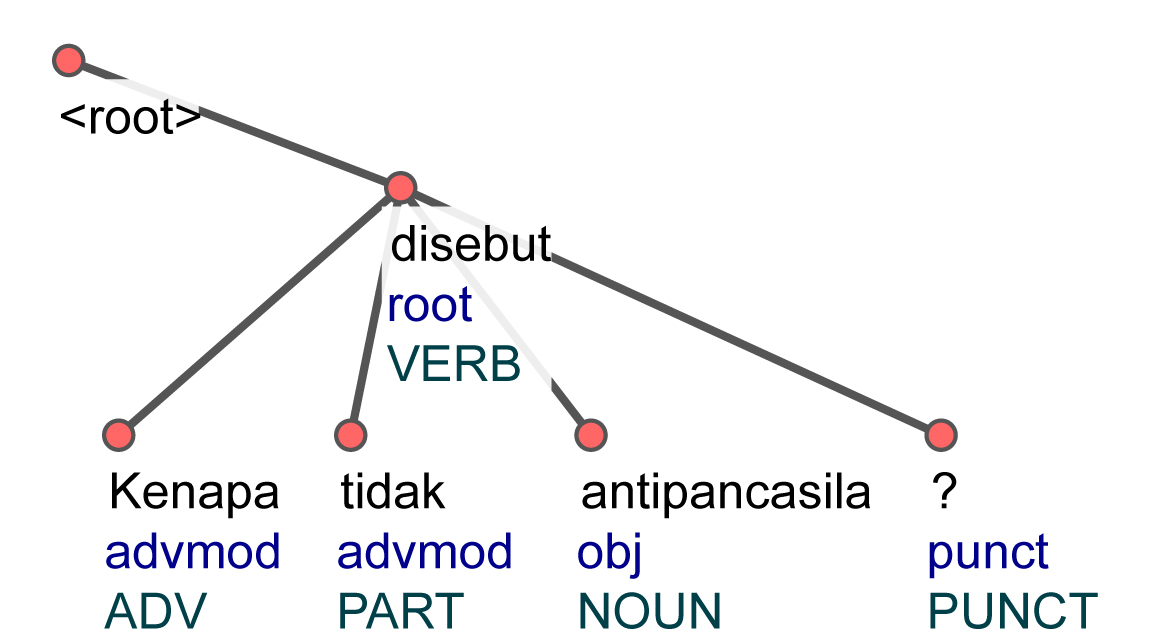
\includegraphics[width=0.8
	\textwidth] {pics/lampiran/lampiranls100.jpg} 
	\caption{lampiranls100} 
	\label{fig:lampiranls100} 
\end{figure}

\begin{figure}
	\centering 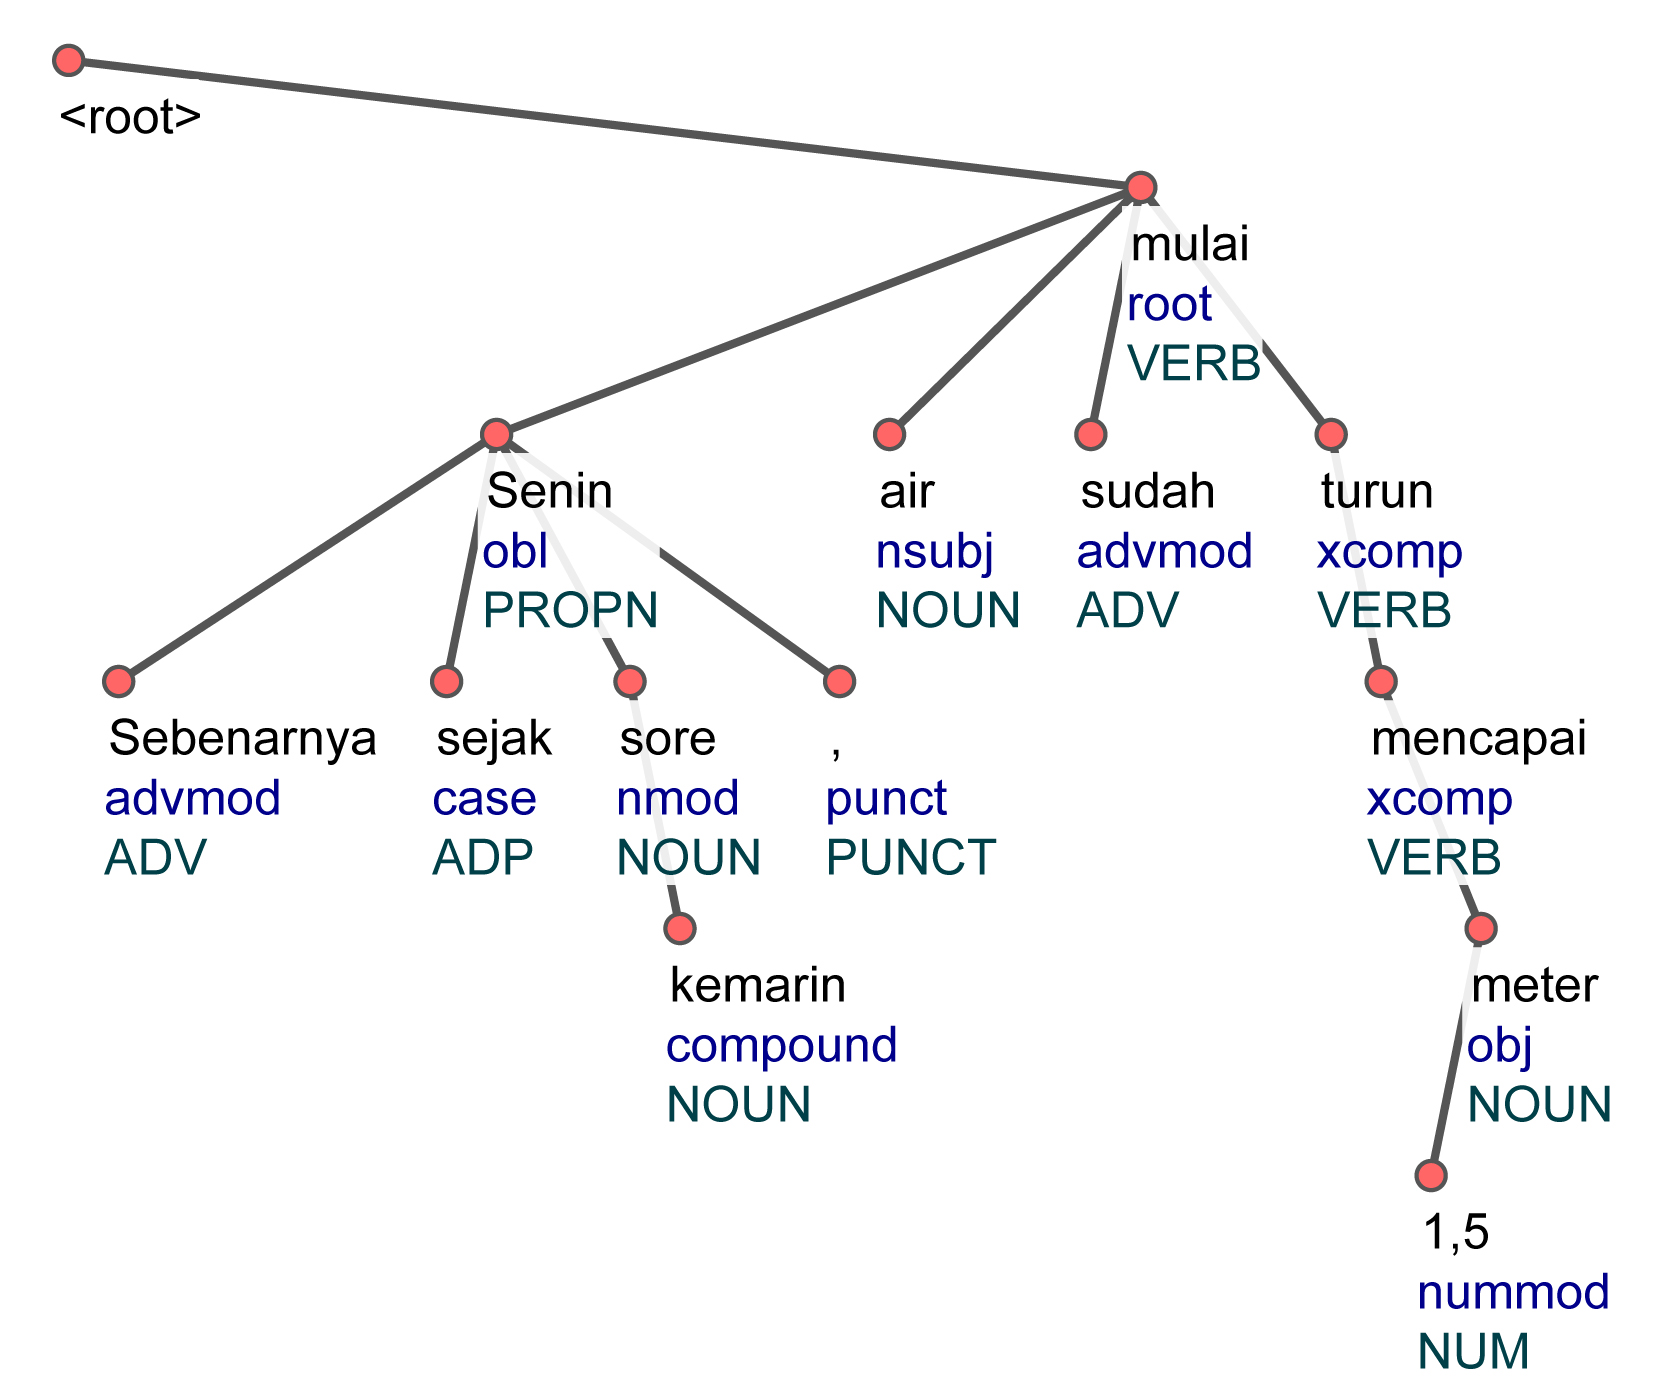
\includegraphics[width=0.8
	\textwidth] {pics/lampiran/lampiranls592.jpg} 
	\caption{lampiranls592} 
	\label{fig:lampiranls592} 
\end{figure}

\begin{figure}
	\centering 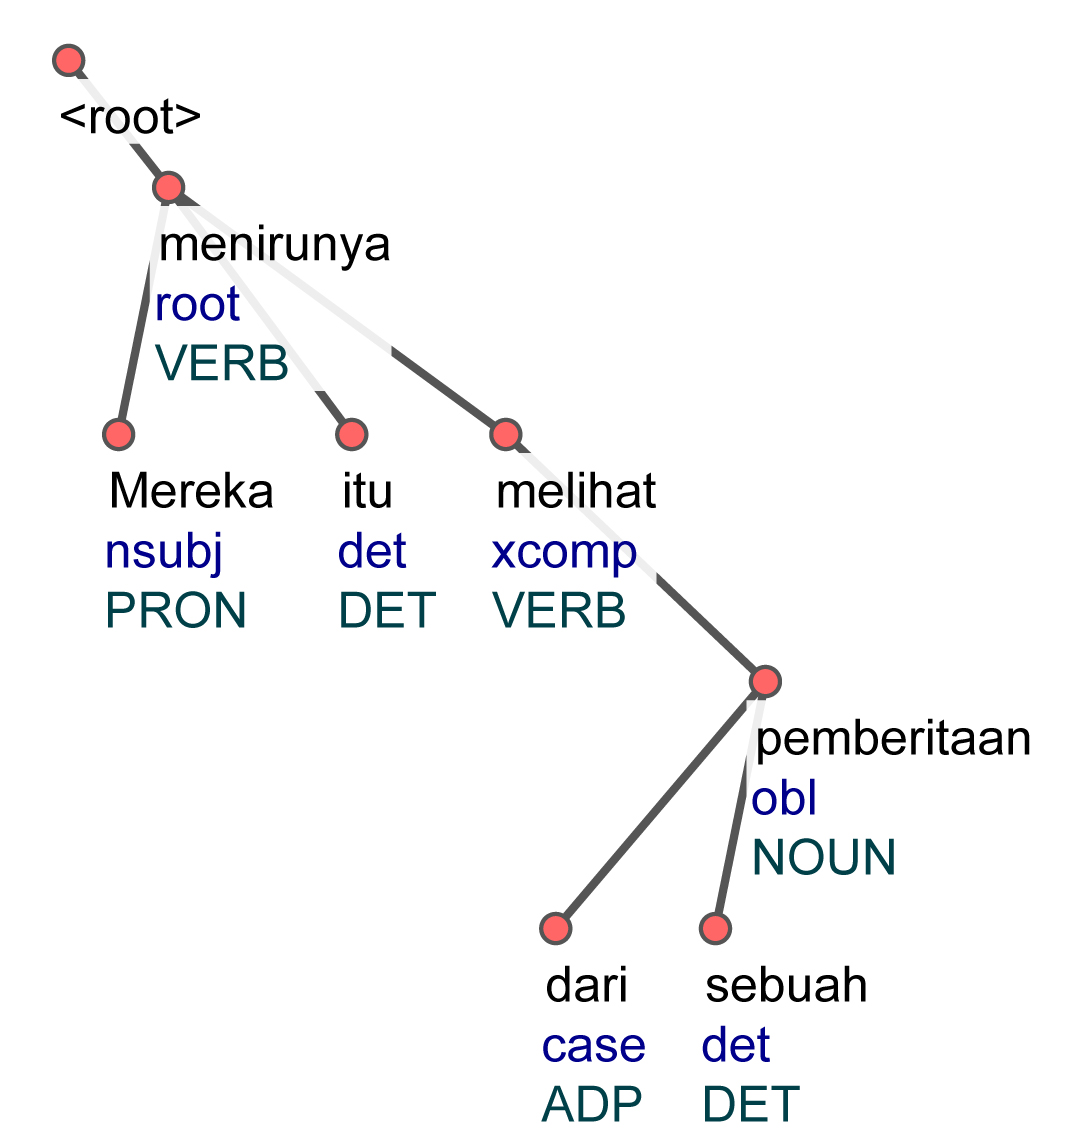
\includegraphics[width=0.8
	\textwidth] {pics/lampiran/lampiranls1100.jpg} 
	\caption{lampiranls1100} 
	\label{fig:lampiranls1100} 
\end{figure}

\begin{figure}
	\centering 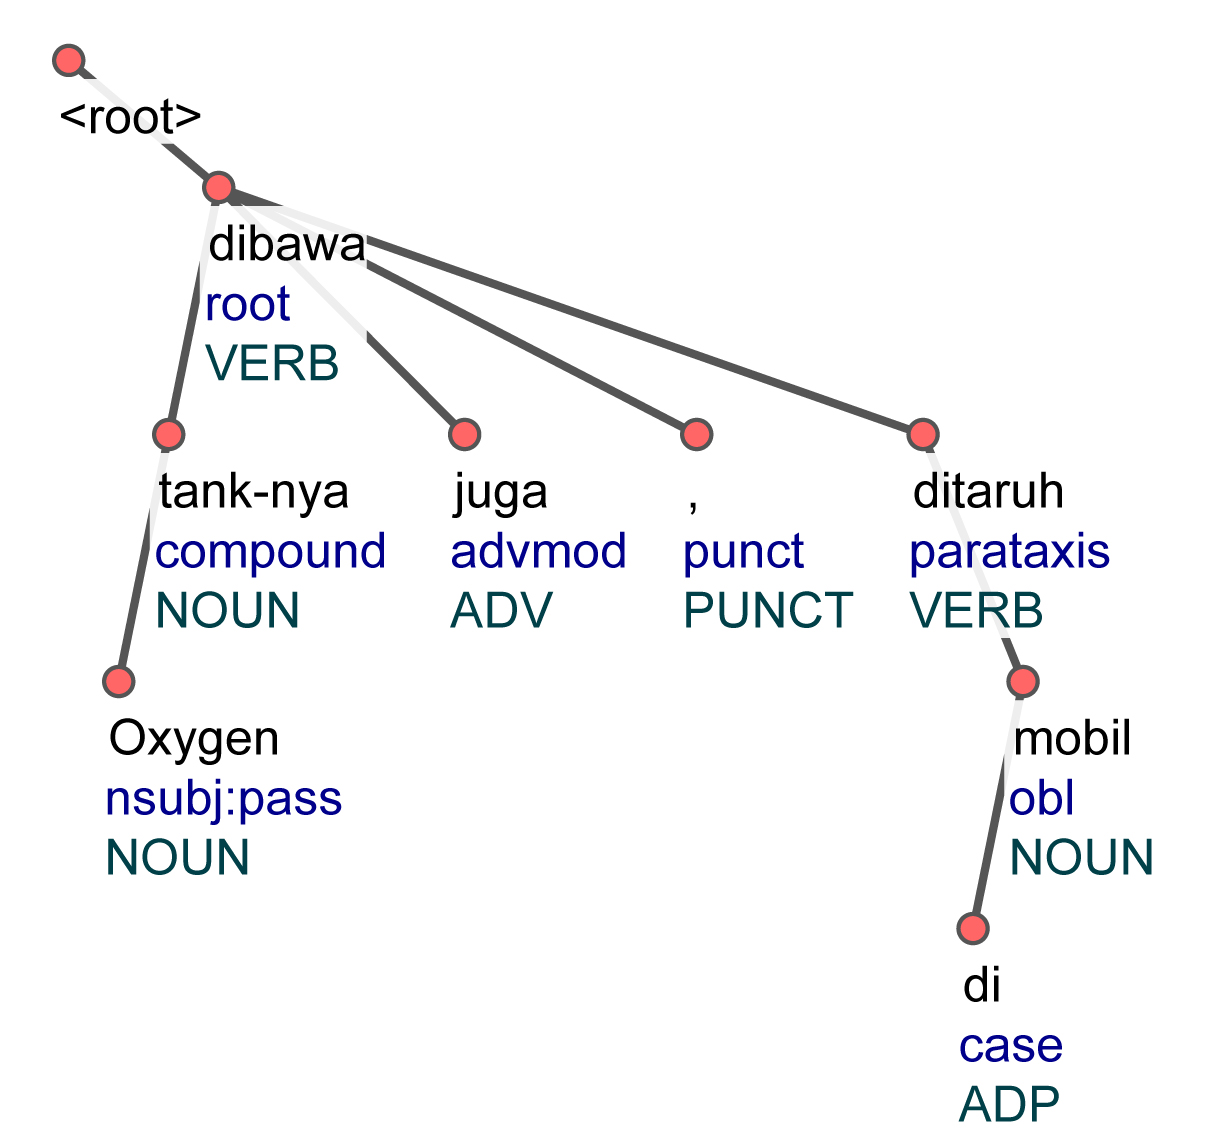
\includegraphics[width=0.8
	\textwidth] {pics/lampiran/lampiranls1836.jpg} 
	\caption{lampiranls1836} 
	\label{fig:lampiranls1836} 
\end{figure}

\begin{figure}
	\centering 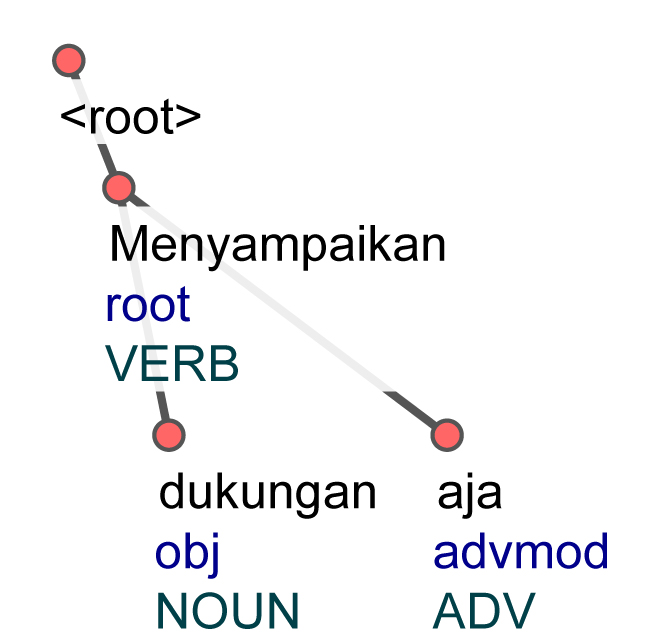
\includegraphics[width=0.8
	\textwidth] {pics/lampiran/lampiranls1928.jpg} 
	\caption{lampiranls1928} 
	\label{fig:lampiranls1928} 
\end{figure}

%%

\begin{figure}
	\centering 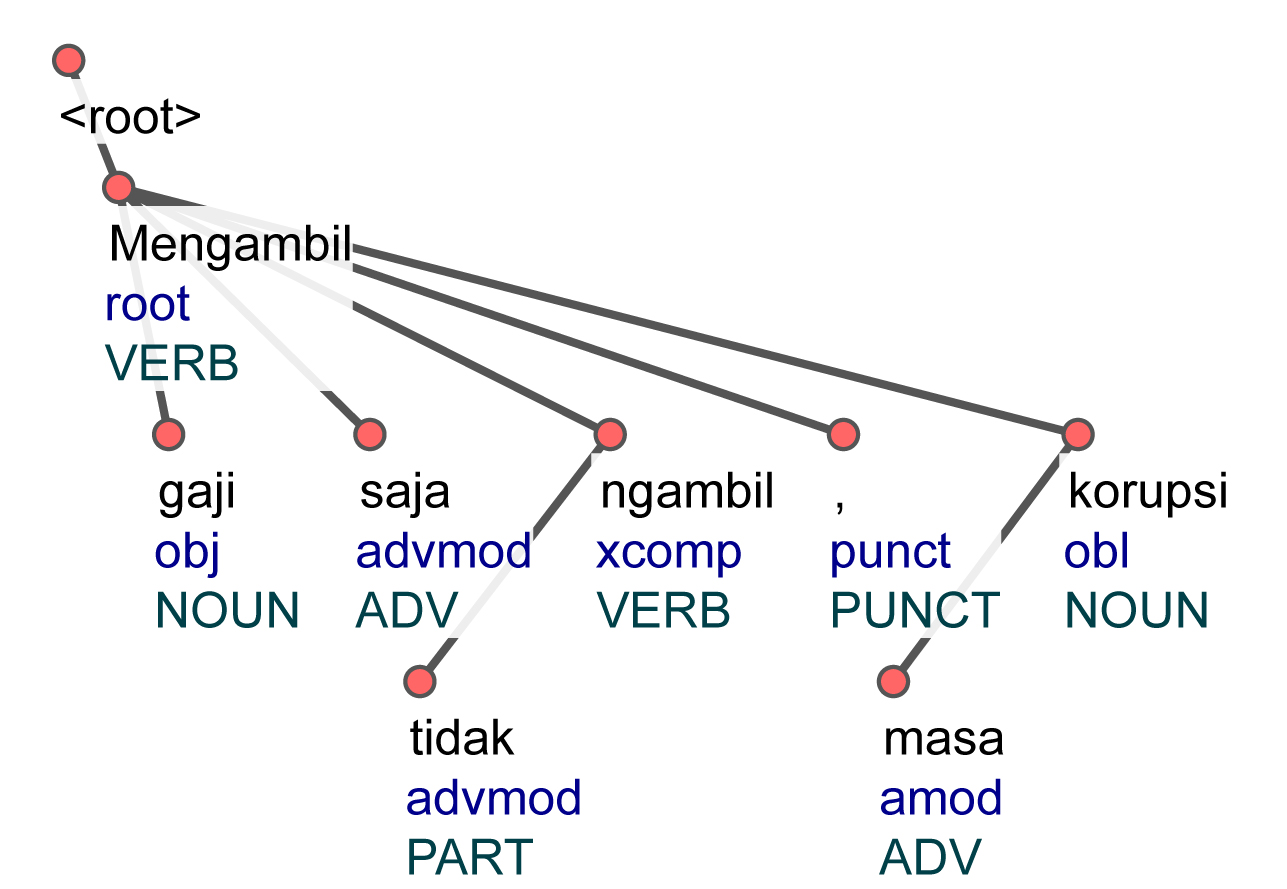
\includegraphics[width=0.8
	\textwidth] {pics/lampiran/lampiranls3530.jpg} 
	\caption{lampiranls3530} 
	\label{fig:lampiranls3530} 
\end{figure}

\begin{figure}
	\centering 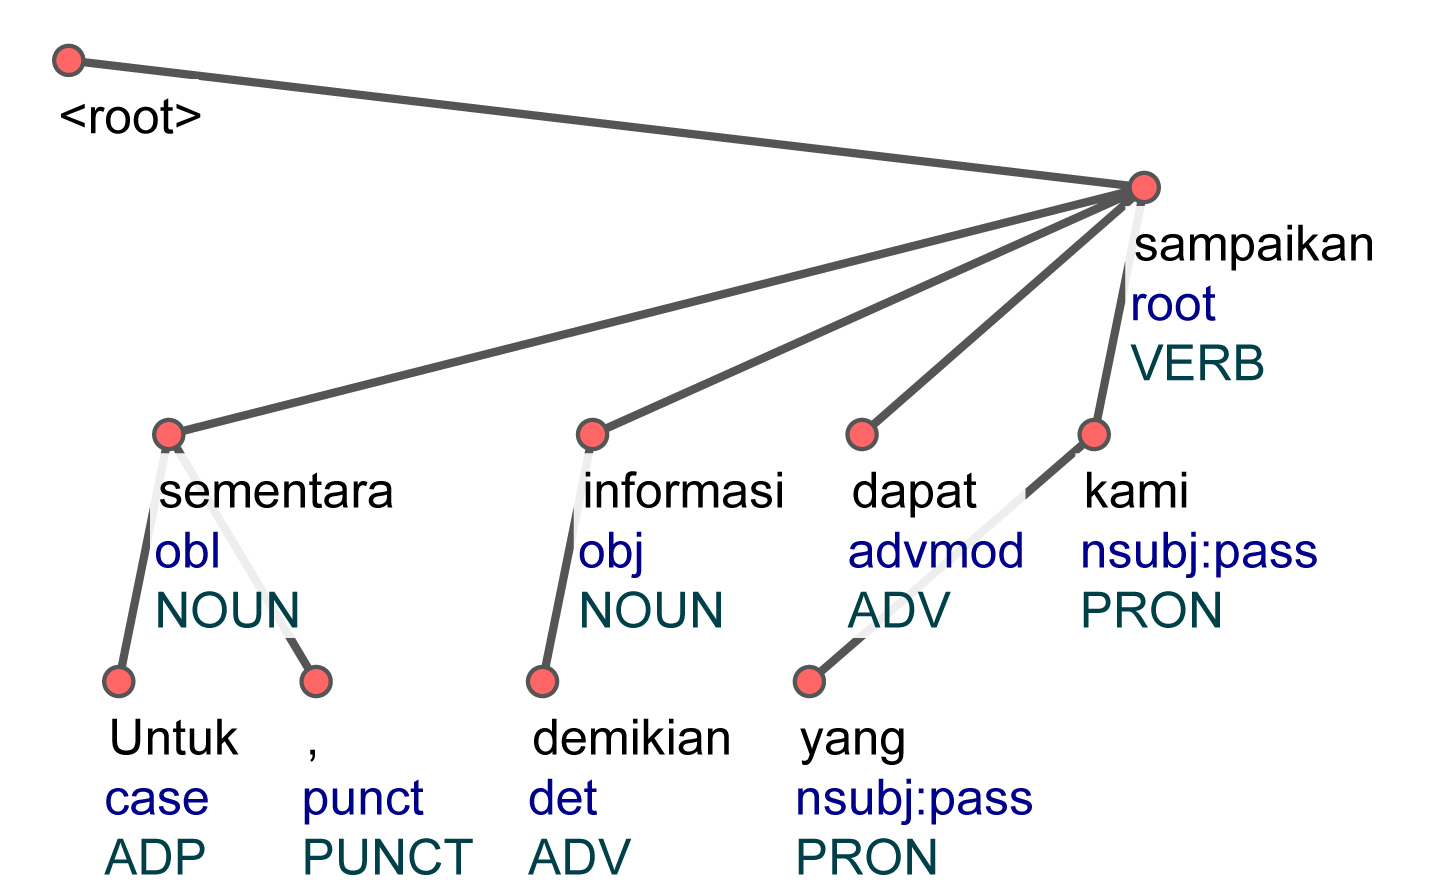
\includegraphics[width=0.8
	\textwidth] {pics/lampiran/lampiranls4327.jpg} 
	\caption{lampiranls4327} 
	\label{fig:lampiranls4327} 
\end{figure}

\begin{figure}
	\centering 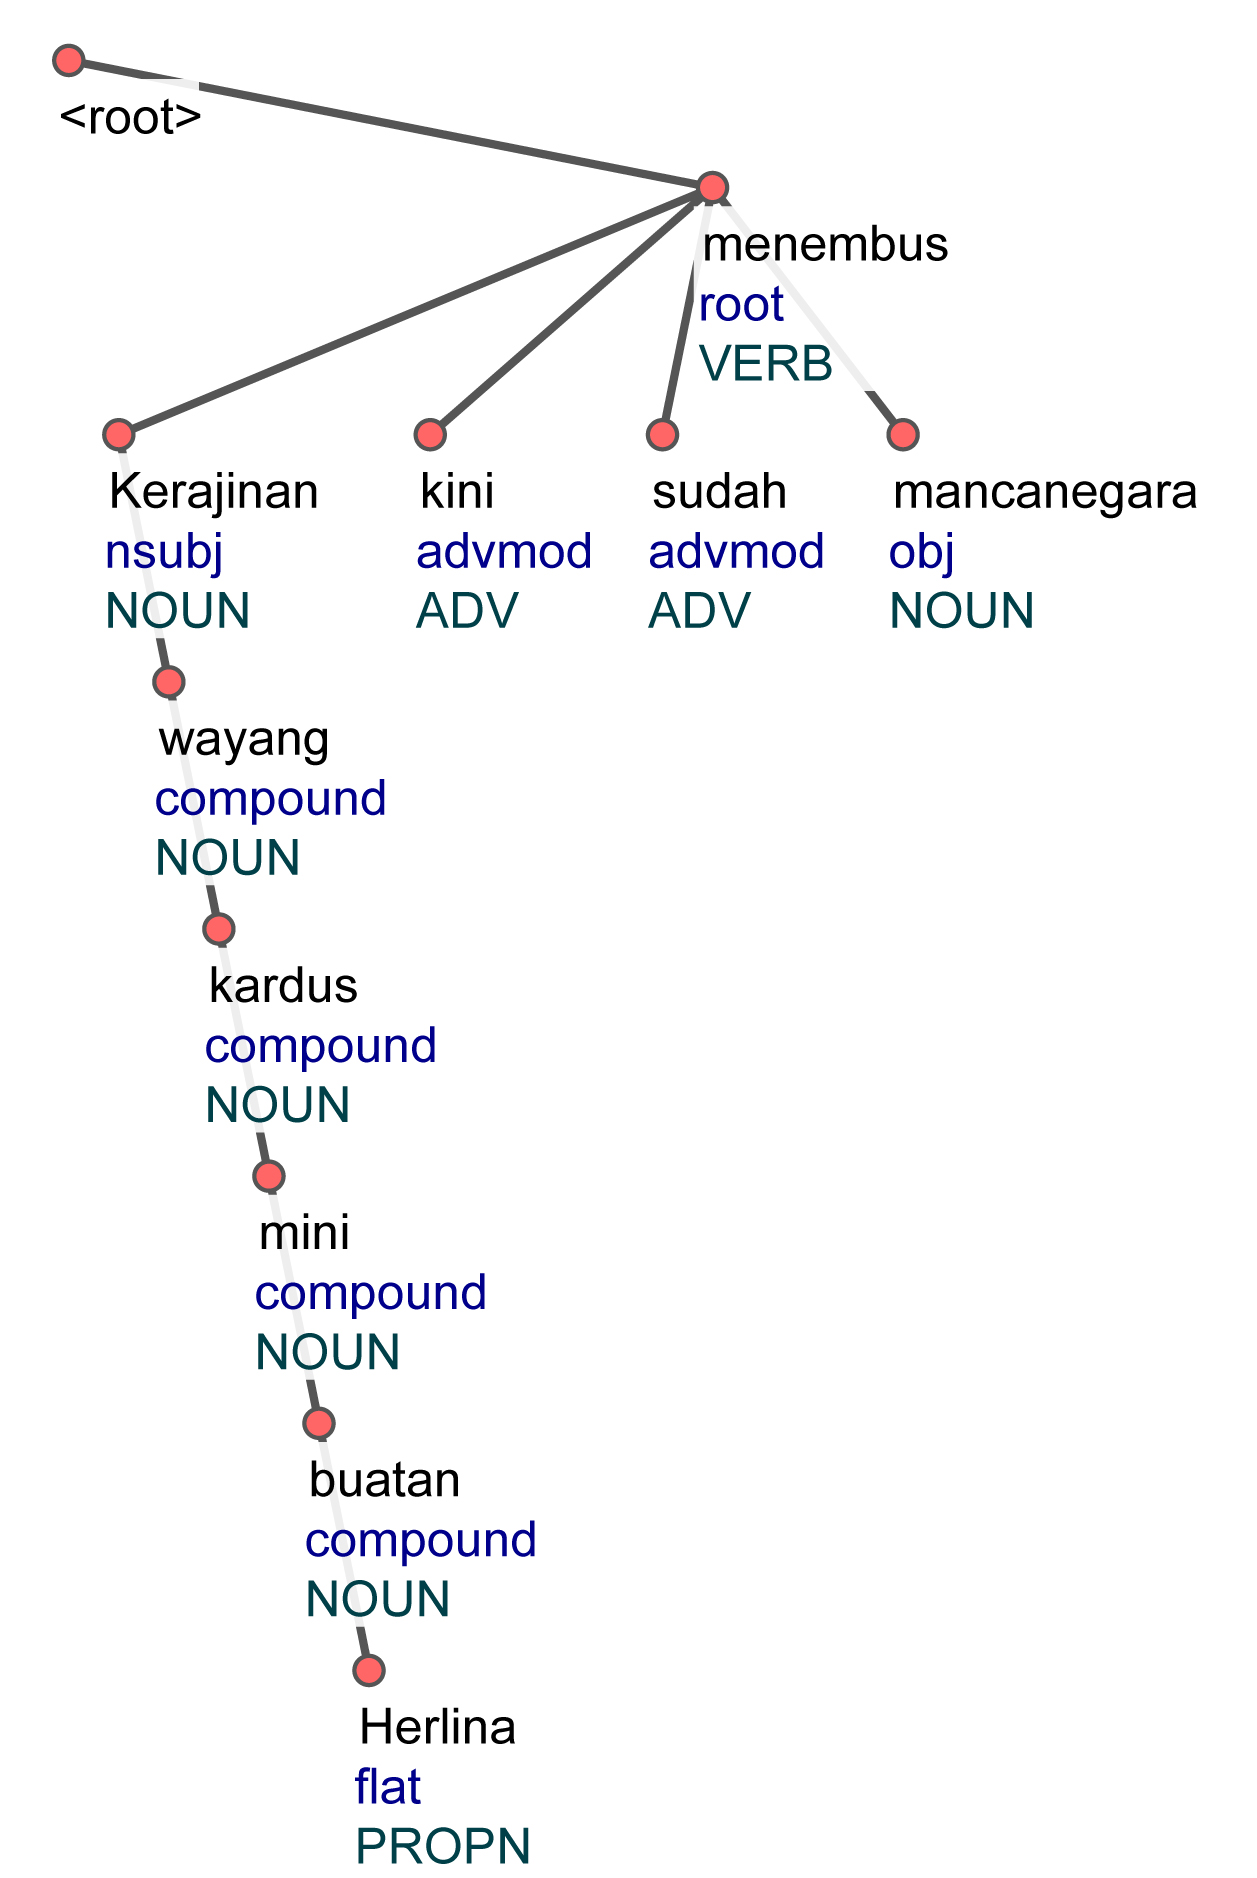
\includegraphics[width=0.8
	\textwidth] {pics/lampiran/lampiranls4991.jpg} 
	\caption{lampiranls4991} 
	\label{fig:lampiranls4991} 
\end{figure}

\begin{figure}
	\centering 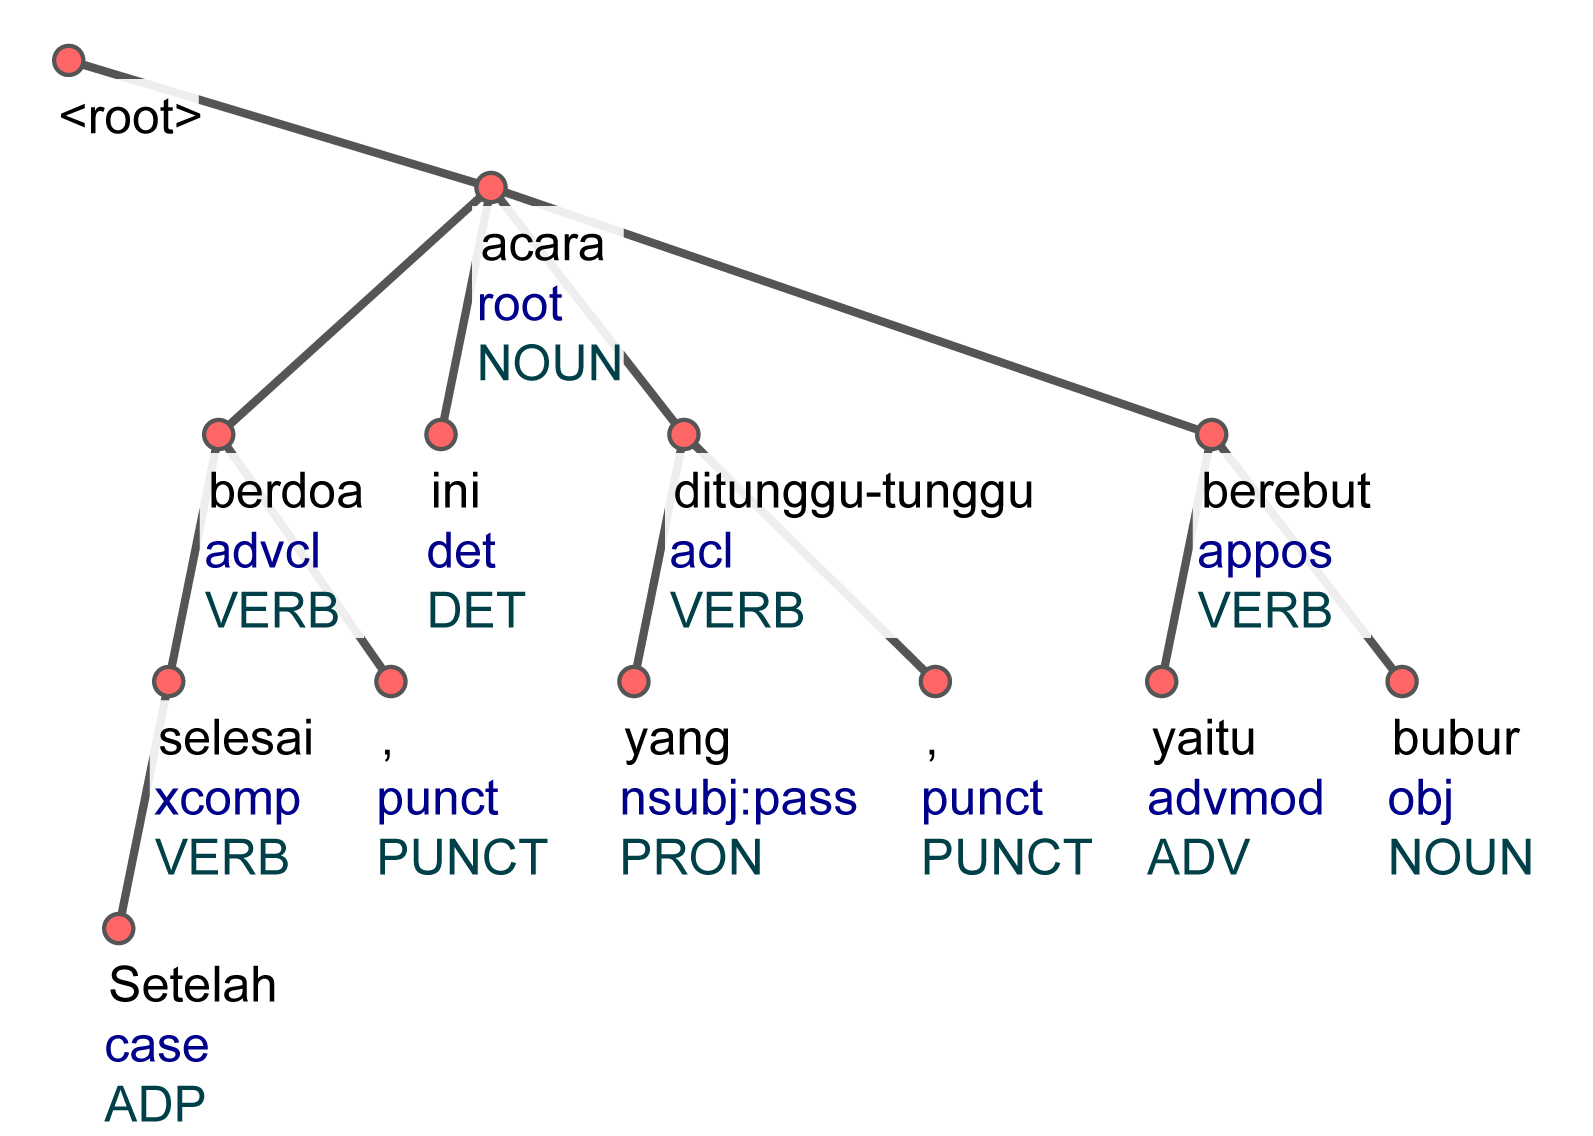
\includegraphics[width=0.8
	\textwidth] {pics/lampiran/lampiranls5677.jpg} 
	\caption{lampiranls5677} 
	\label{fig:lampiranls5677} 
\end{figure}

\begin{figure}
	\centering 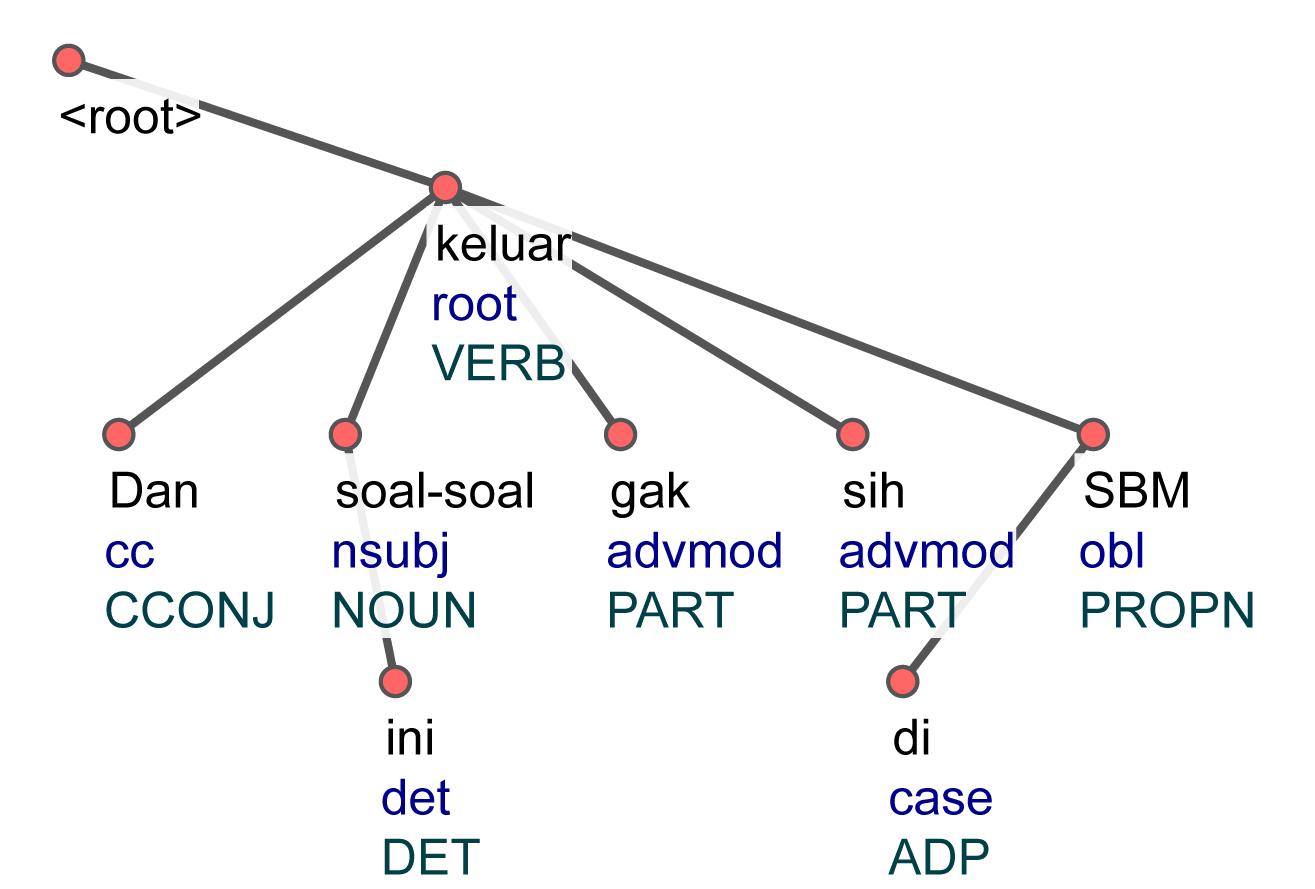
\includegraphics[width=0.8
	\textwidth] {pics/lampiran/lampiranls7047.jpg} 
	\caption{lampiranls7047} 
	\label{fig:lampiranls7047} 
\end{figure}

%%

\begin{figure}
	\centering 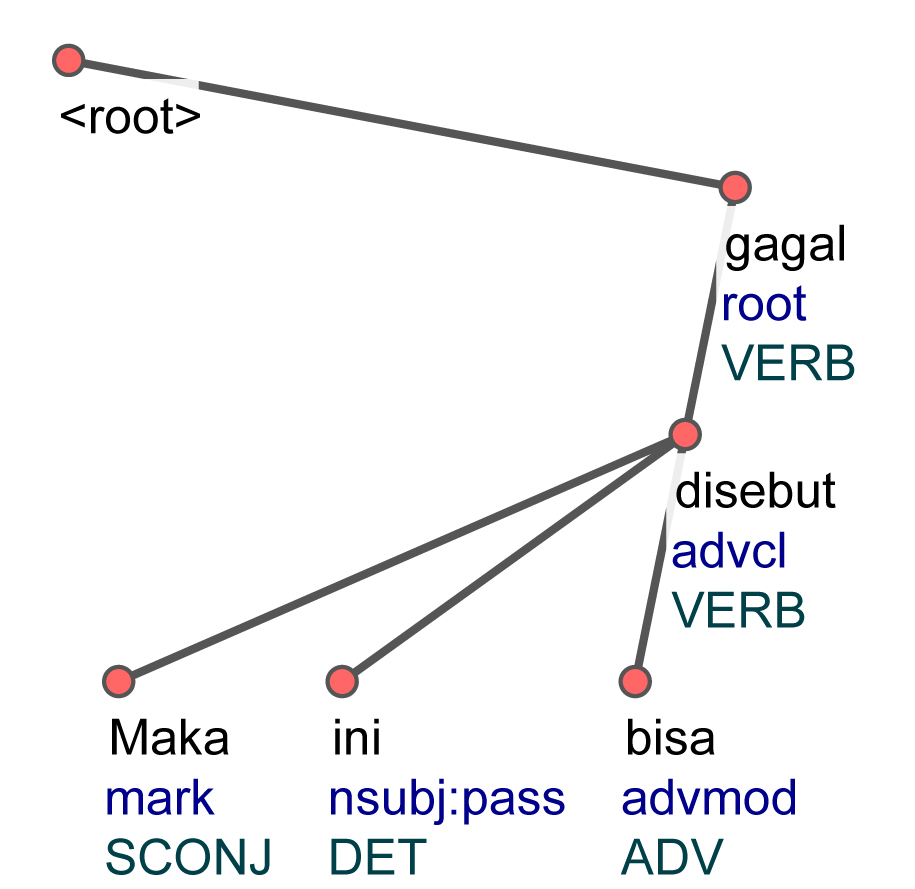
\includegraphics[width=0.8
	\textwidth] {pics/lampiran/lampiranls7359.jpg} 
	\caption{lampiranls7359} 
	\label{fig:lampiranls7359} 
\end{figure}

\begin{figure}
	\centering 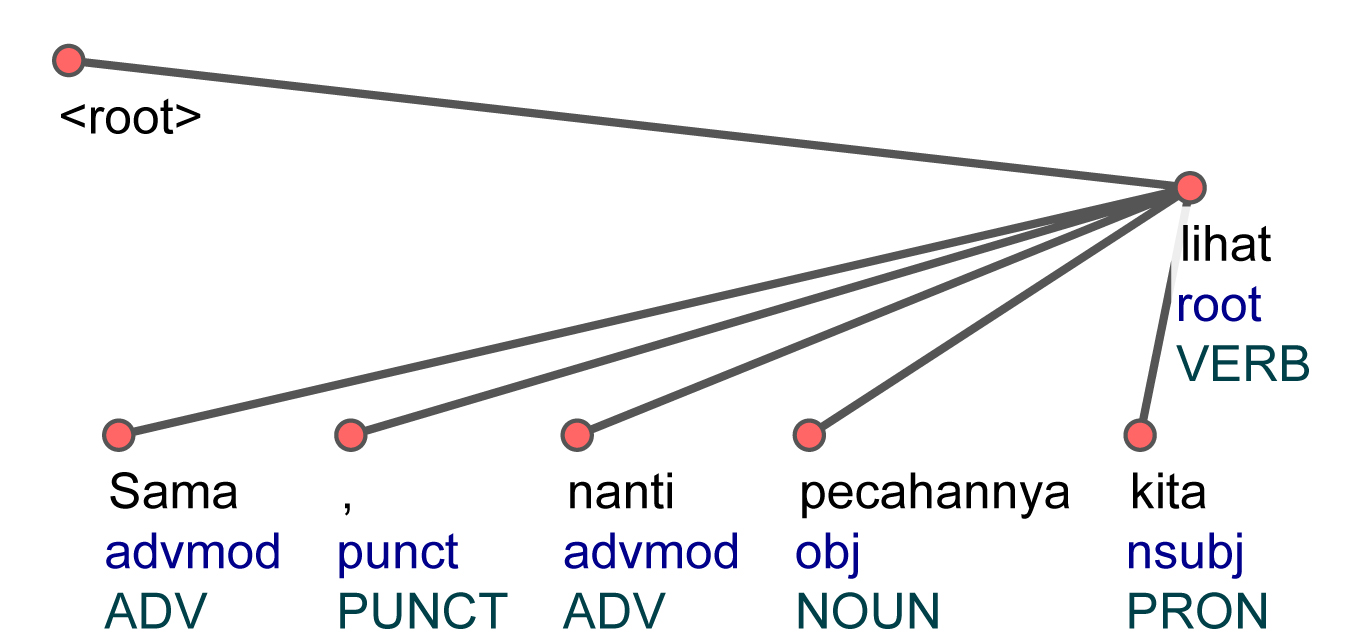
\includegraphics[width=0.8
	\textwidth] {pics/lampiran/lampiranls7375.jpg} 
	\caption{lampiranls7375} 
	\label{fig:lampiranls7375} 
\end{figure}

%% TS

\begin{figure}
	\centering 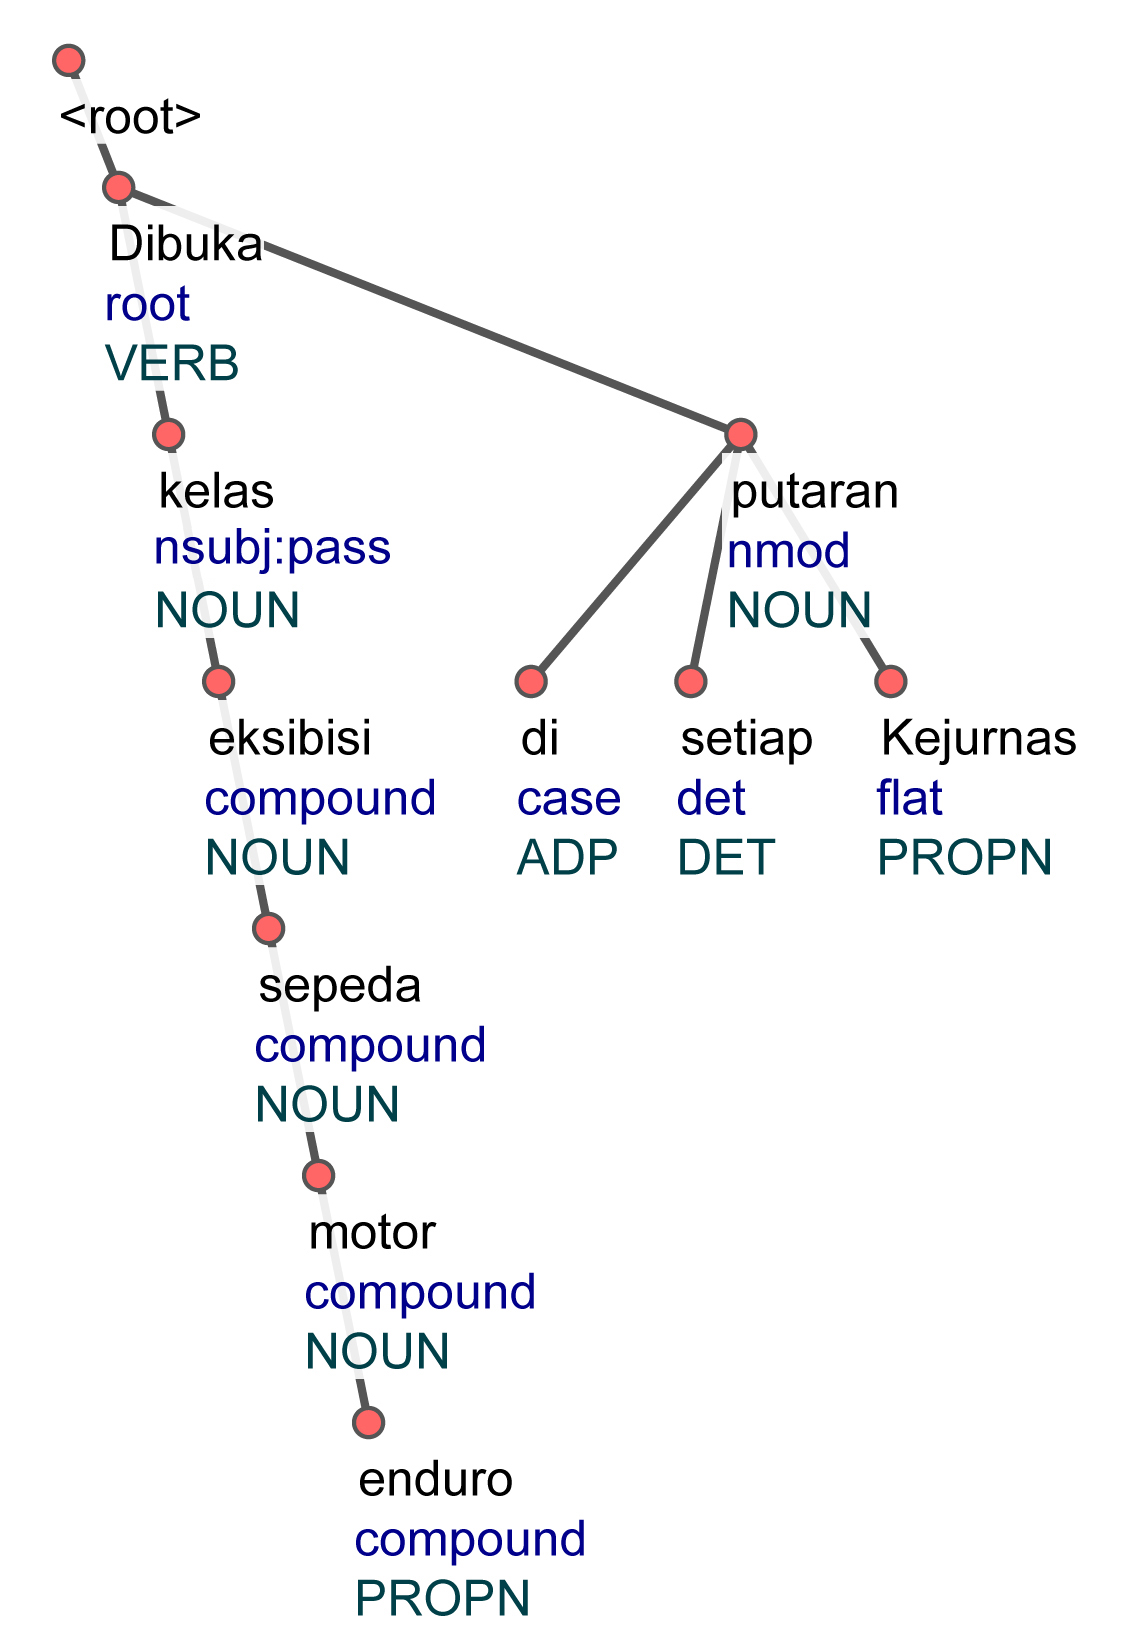
\includegraphics[width=0.8
	\textwidth] {pics/lampiran/lampirants770.jpg} 
	\caption{lampirants770} 
	\label{fig:lampirants770} 
\end{figure}

\begin{figure}
	\centering 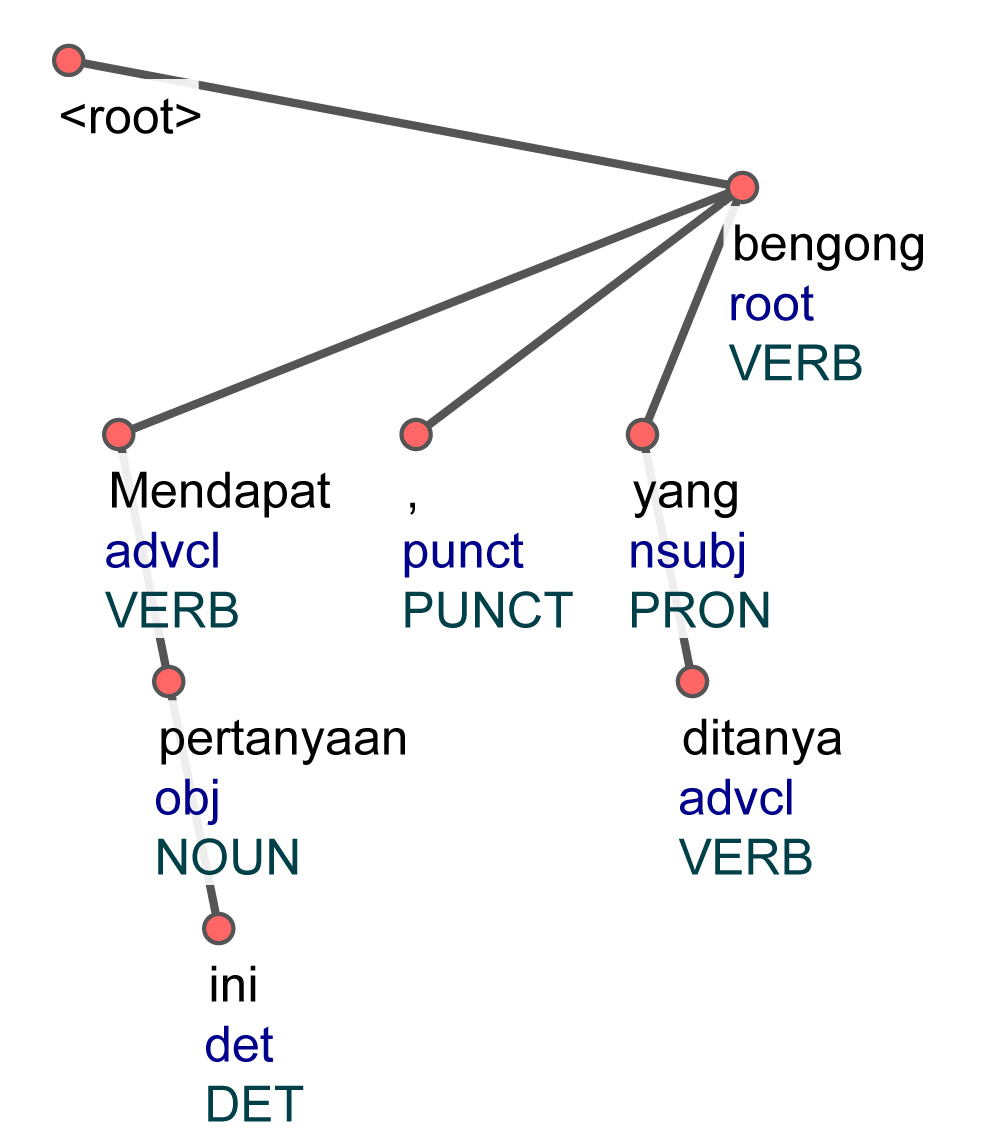
\includegraphics[width=0.8
	\textwidth] {pics/lampiran/lampirants1956.jpg} 
	\caption{lampirants1956} 
	\label{fig:lampirants1956} 
\end{figure}

\begin{figure}
	\centering 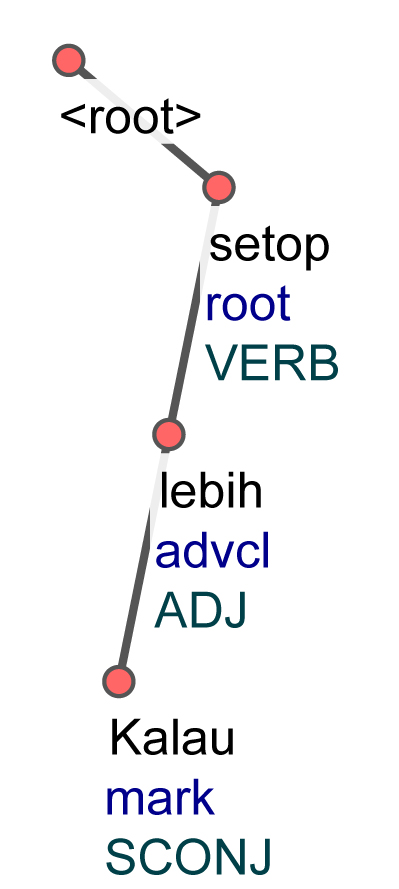
\includegraphics[width=0.8
	\textwidth] {pics/lampiran/lampirants2537.jpg} 
	\caption{lampirants2537} 
	\label{fig:lampirants2537} 
\end{figure}

\begin{figure}
	\centering 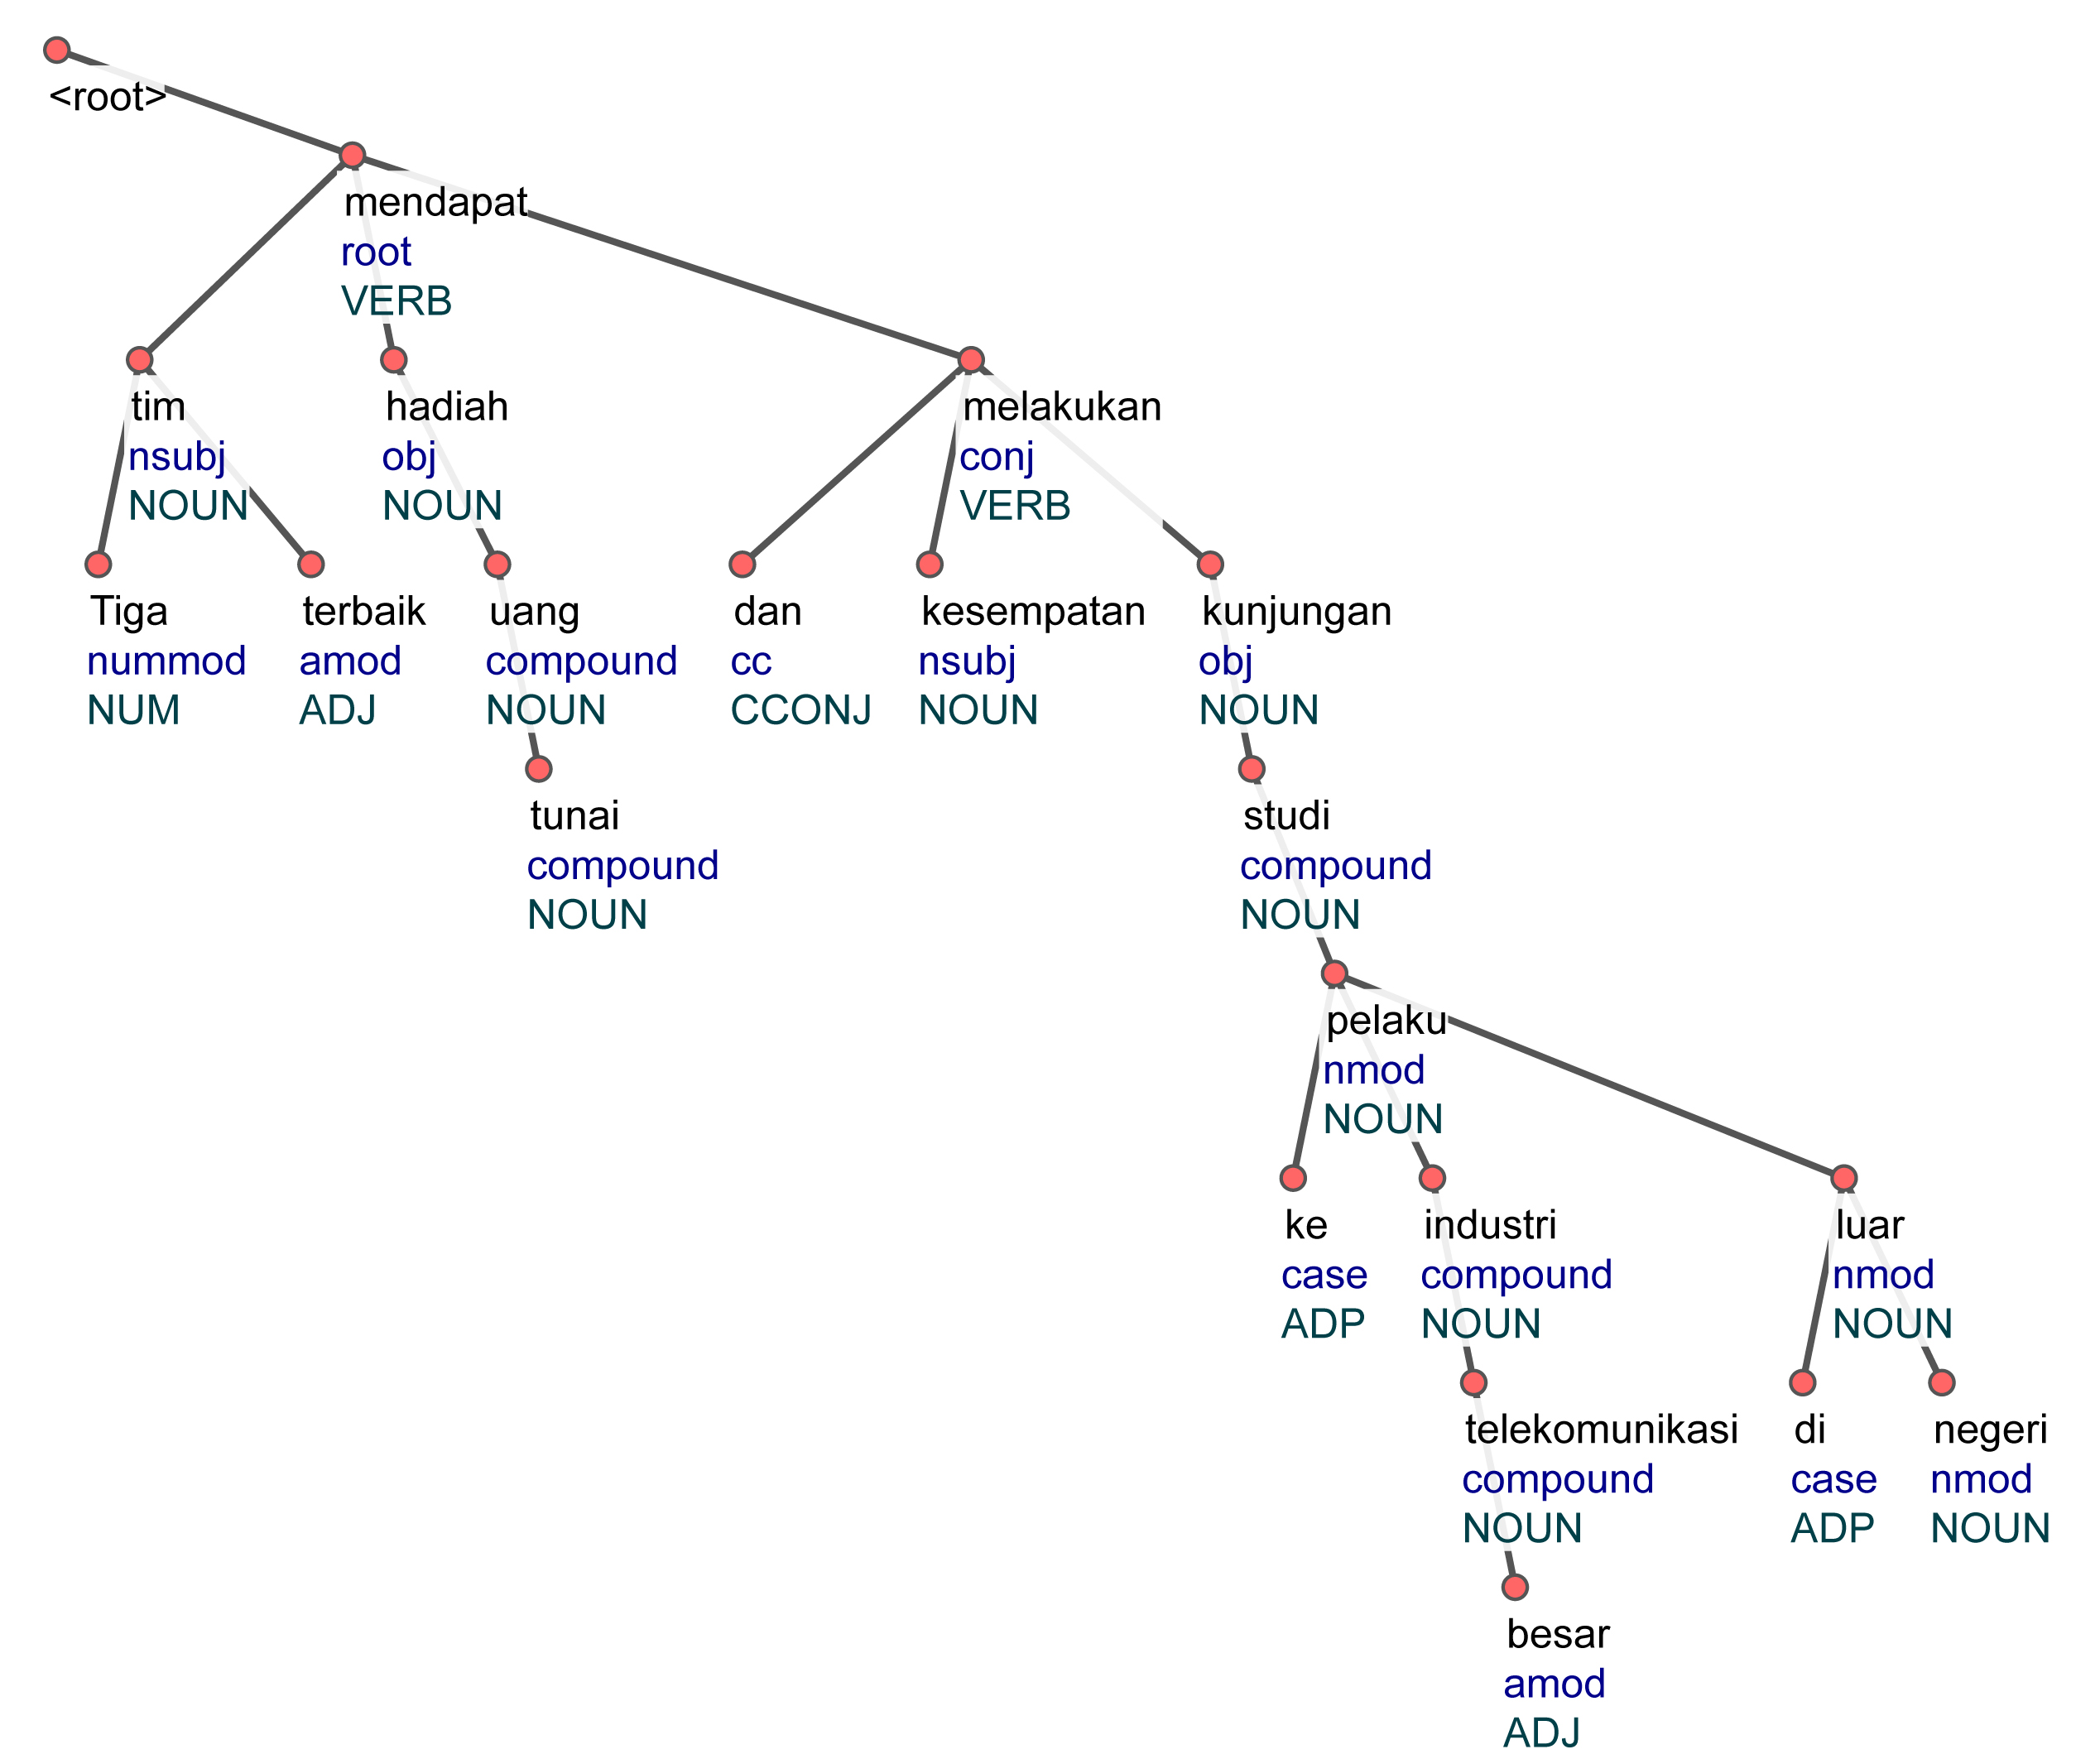
\includegraphics[width=0.8
	\textwidth] {pics/lampiran/lampirants2624.jpg} 
	\caption{lampirants2624} 
	\label{fig:lampirants2624} 
\end{figure}

\begin{figure}
	\centering 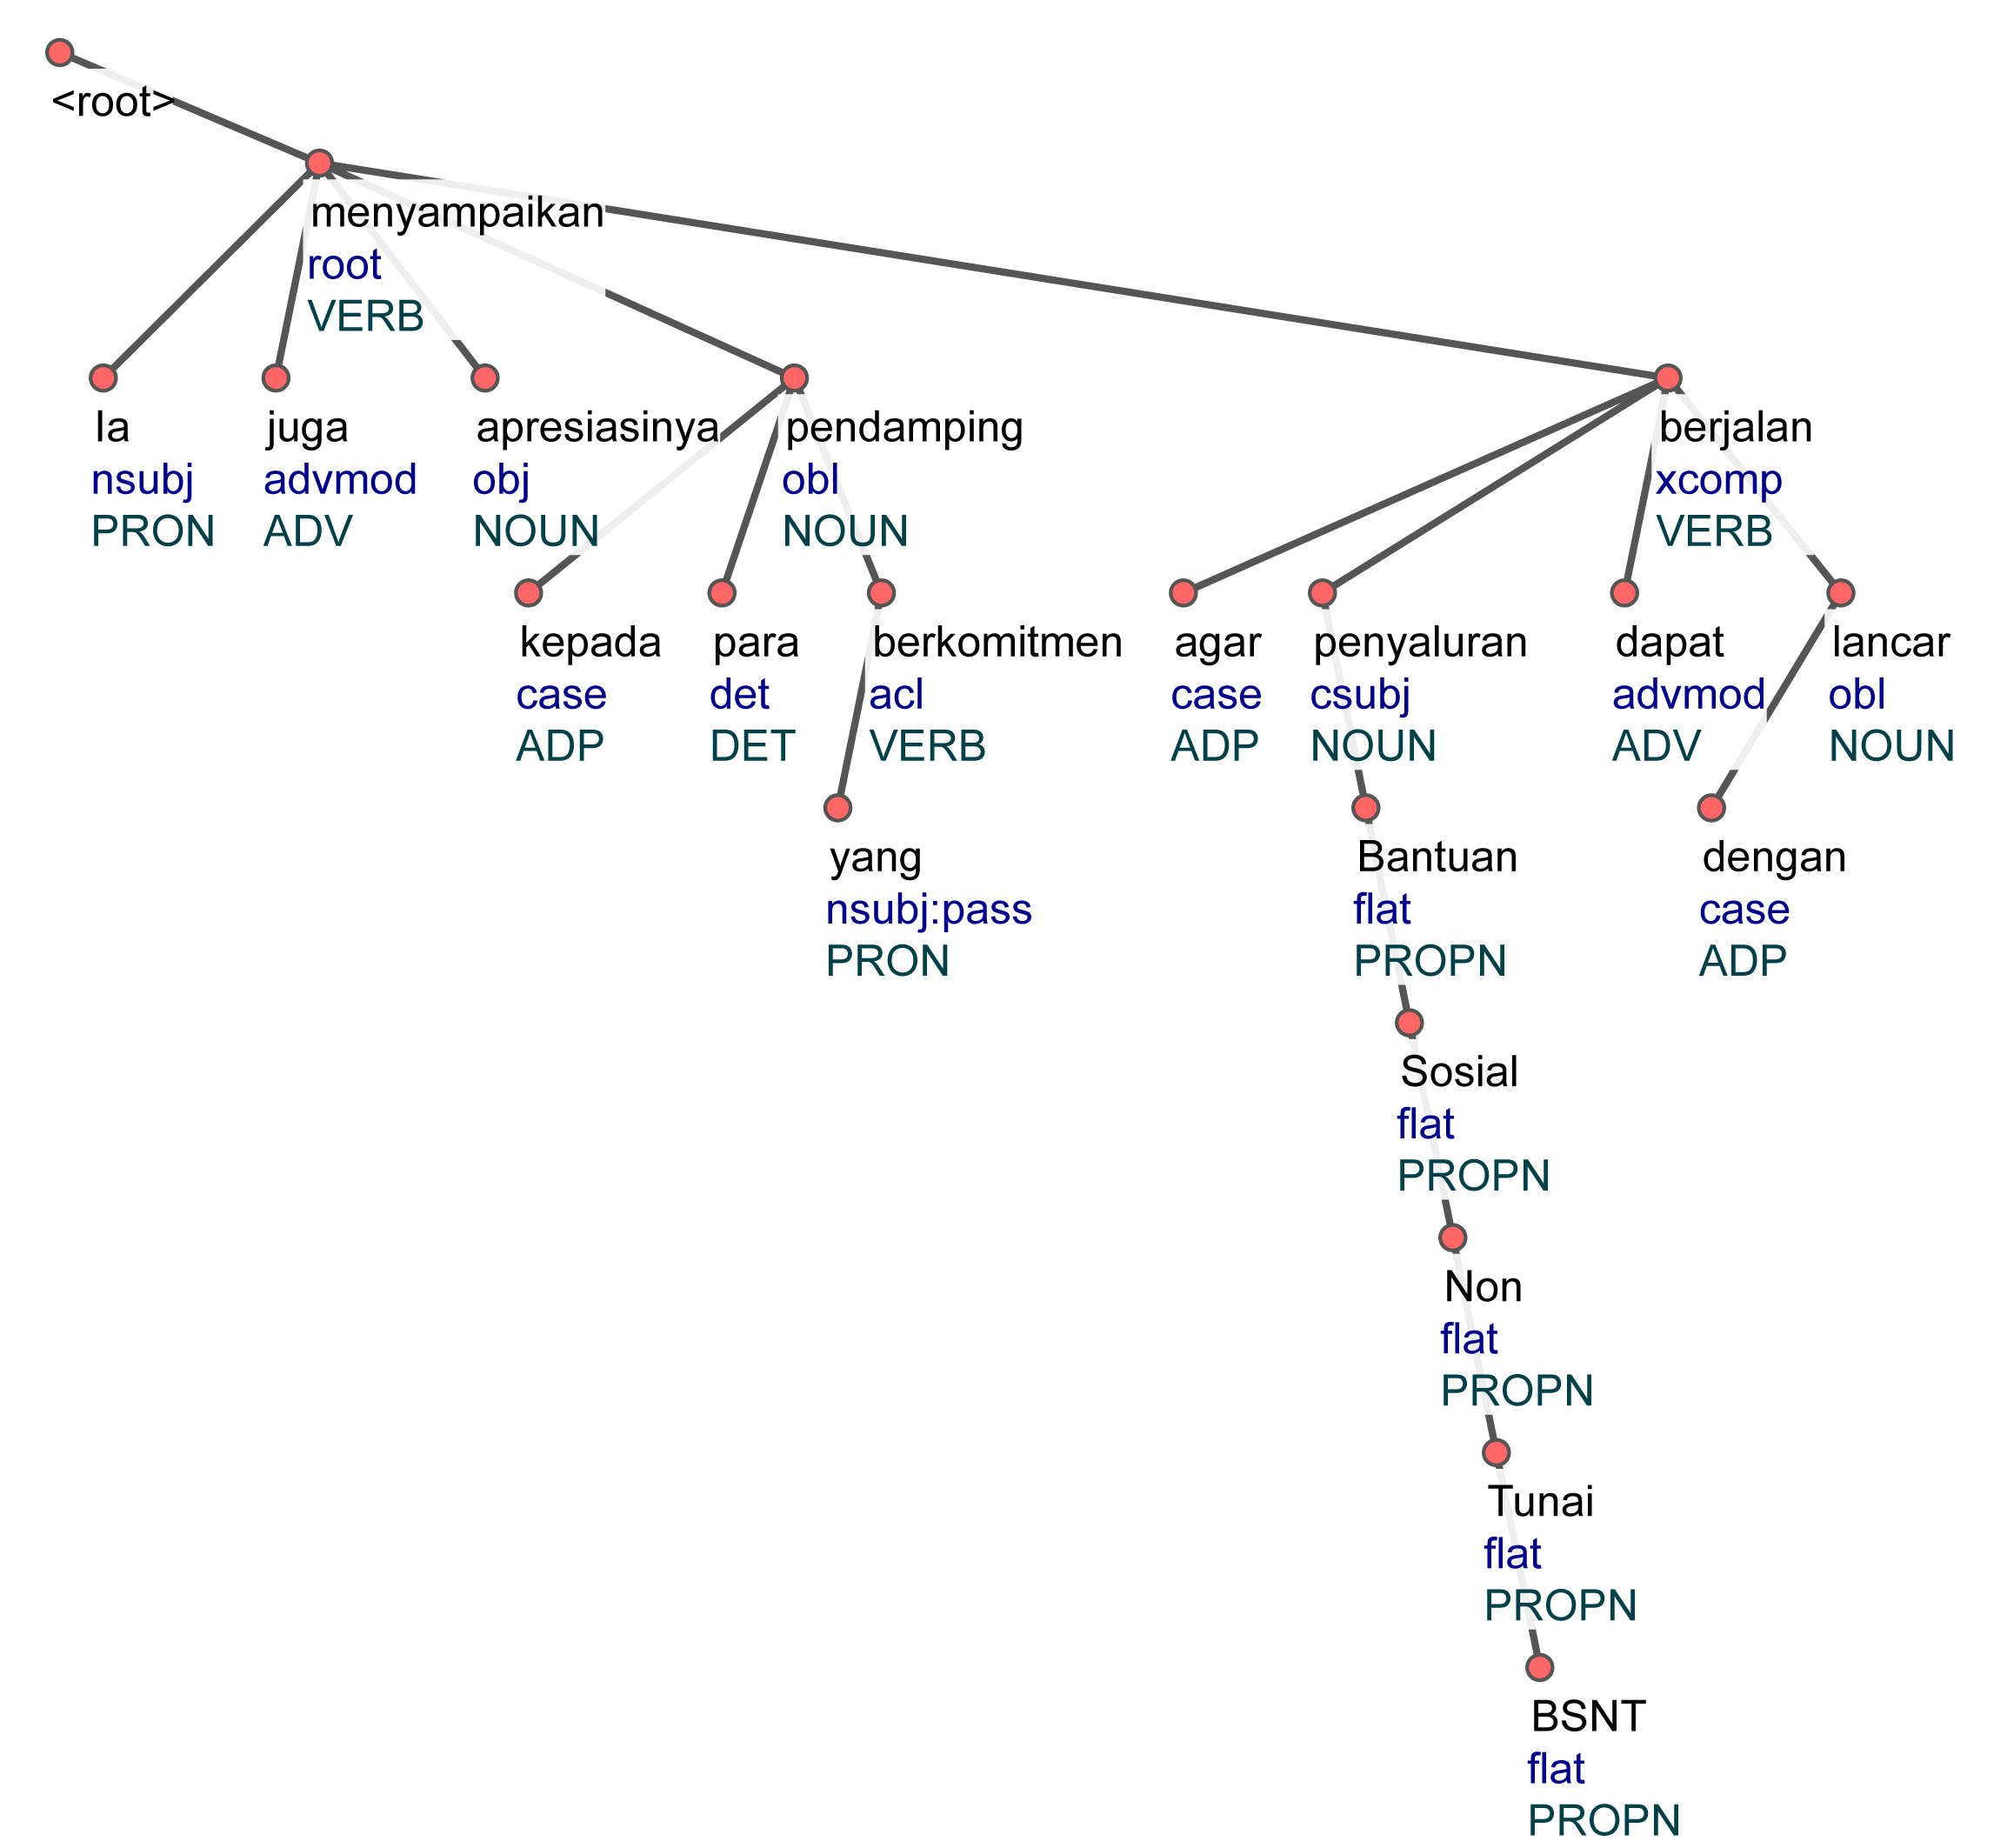
\includegraphics[width=0.8
	\textwidth] {pics/lampiran/lampirants3221.jpg} 
	\caption{lampirants3221} 
	\label{fig:lampirants3221} 
\end{figure}

%%

\begin{figure}
	\centering 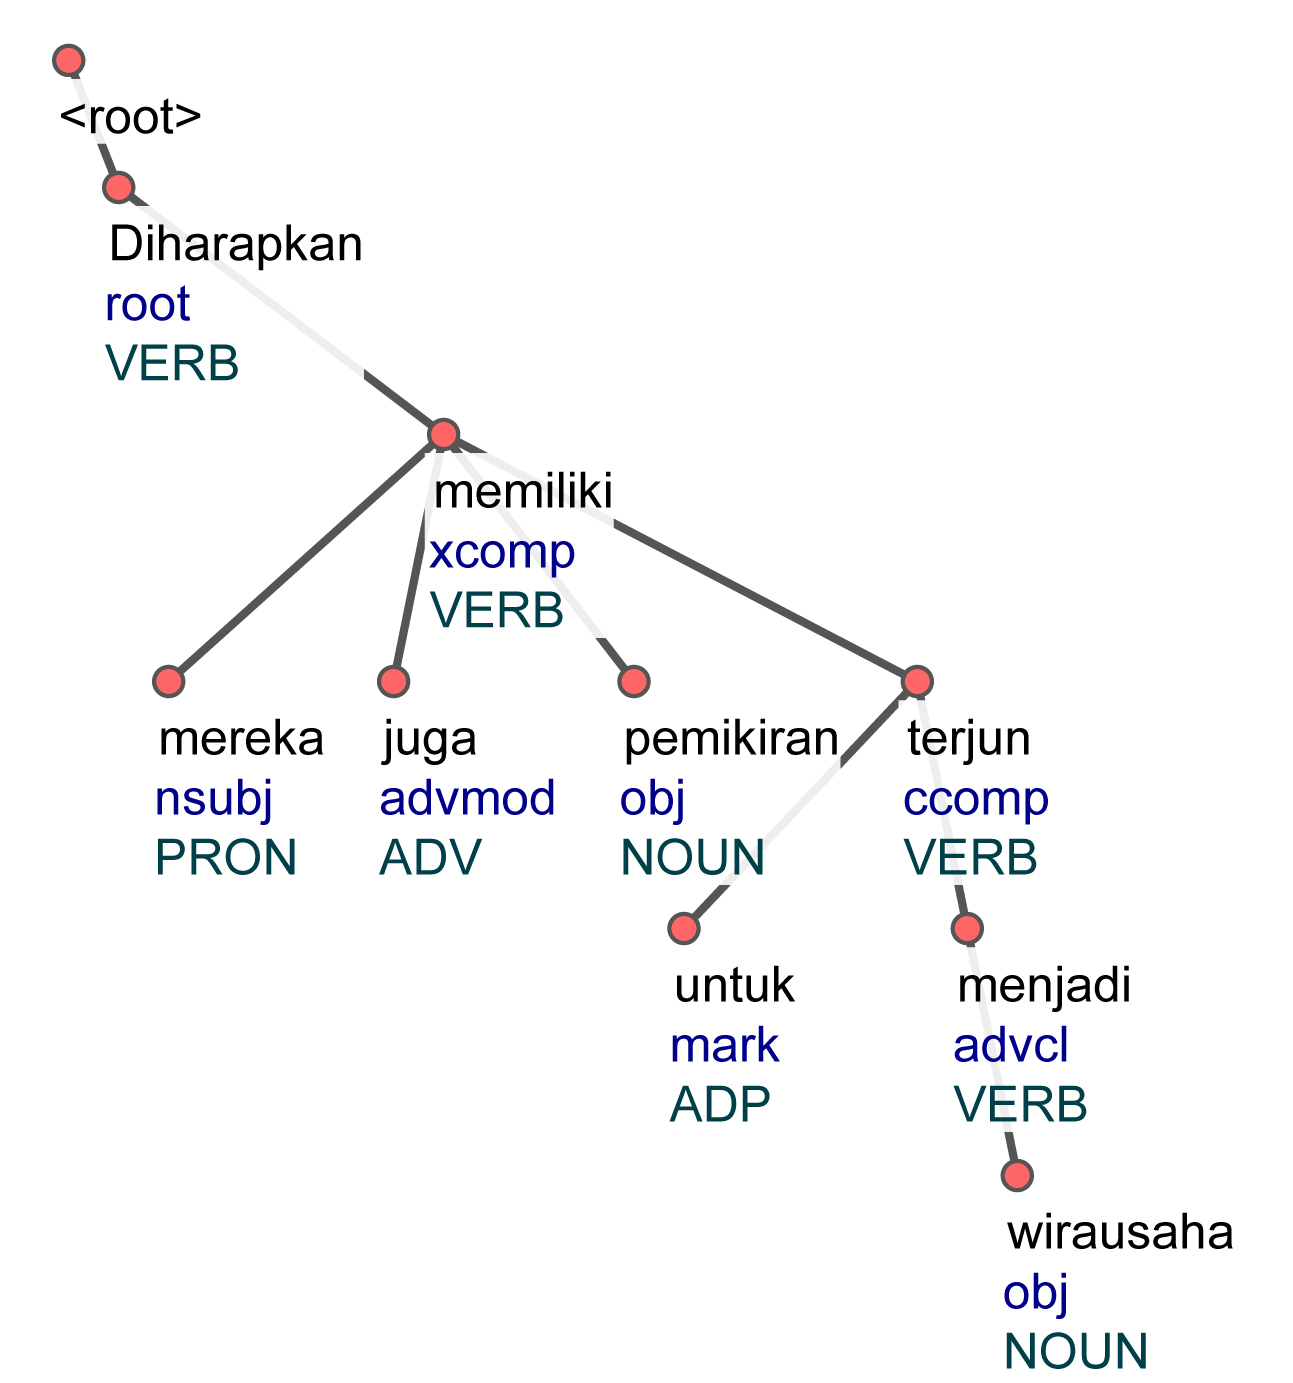
\includegraphics[width=0.8
	\textwidth] {pics/lampiran/lampirants4955.jpg} 
	\caption{lampirants4955} 
	\label{fig:lampirants4955} 
\end{figure}

\begin{figure}
	\centering 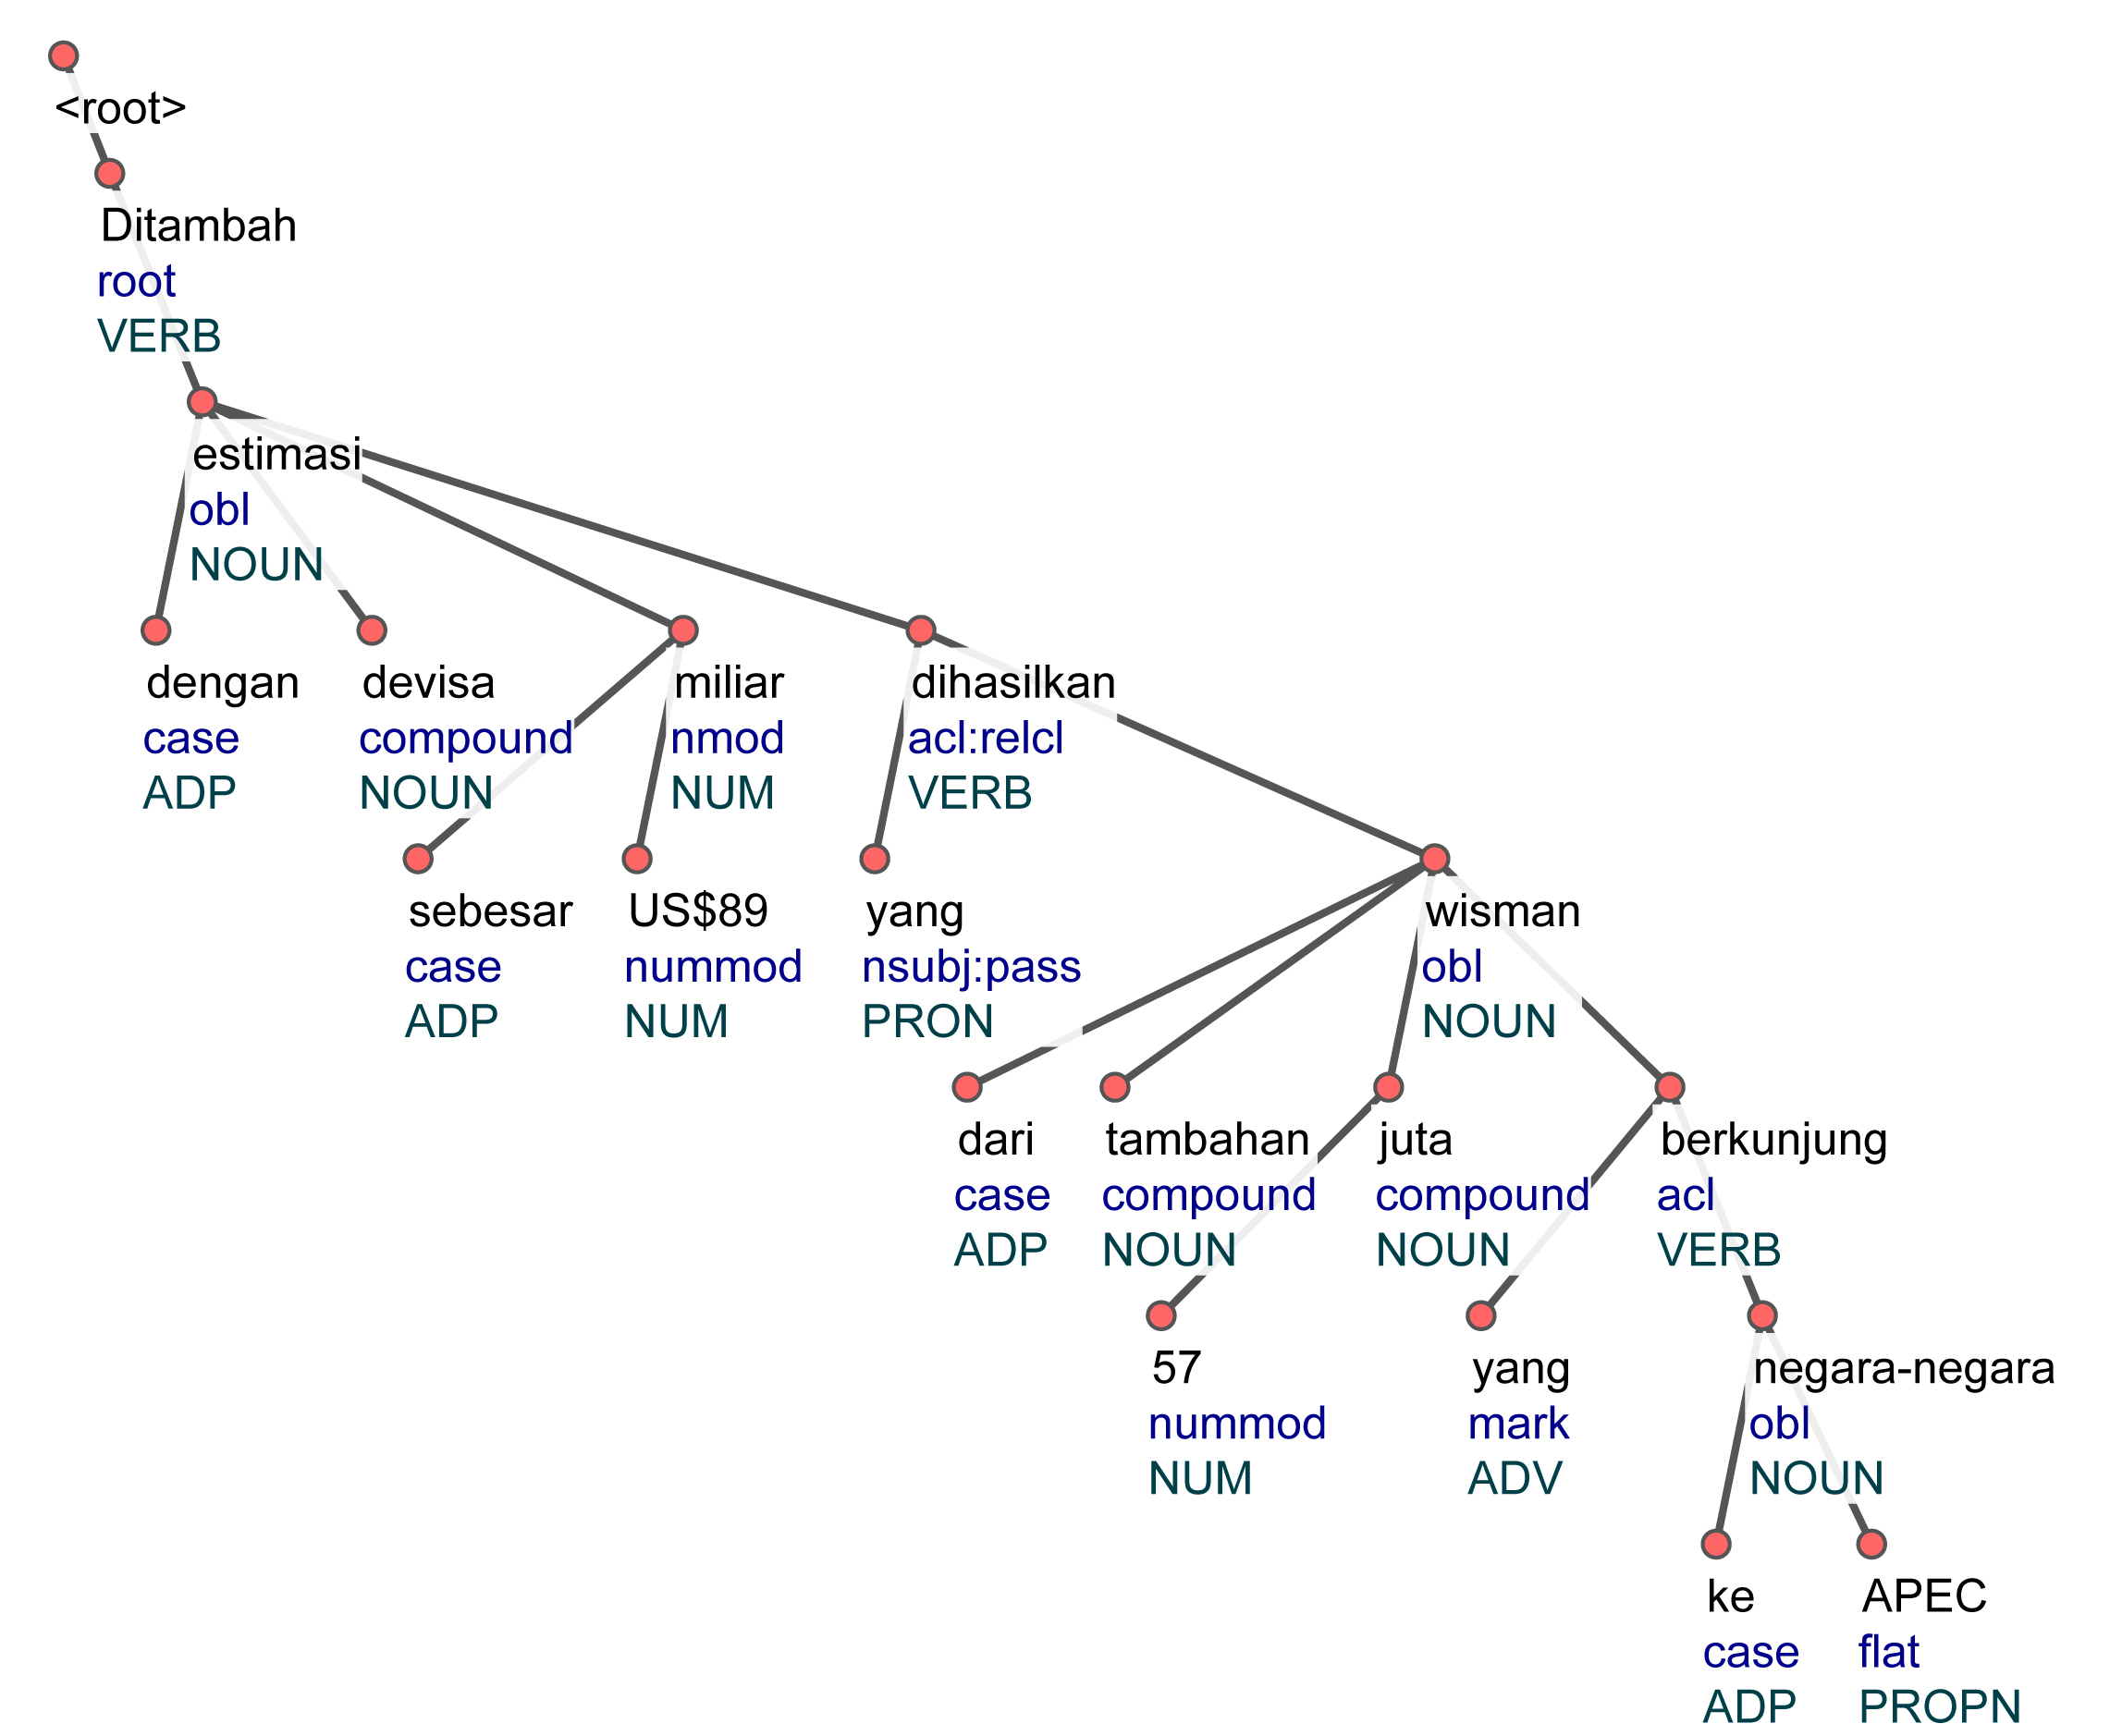
\includegraphics[width=0.8
	\textwidth] {pics/lampiran/lampirants5360.jpg} 
	\caption{lampirants5360} 
	\label{fig:lampirants5360} 
\end{figure}

\begin{figure}
	\centering 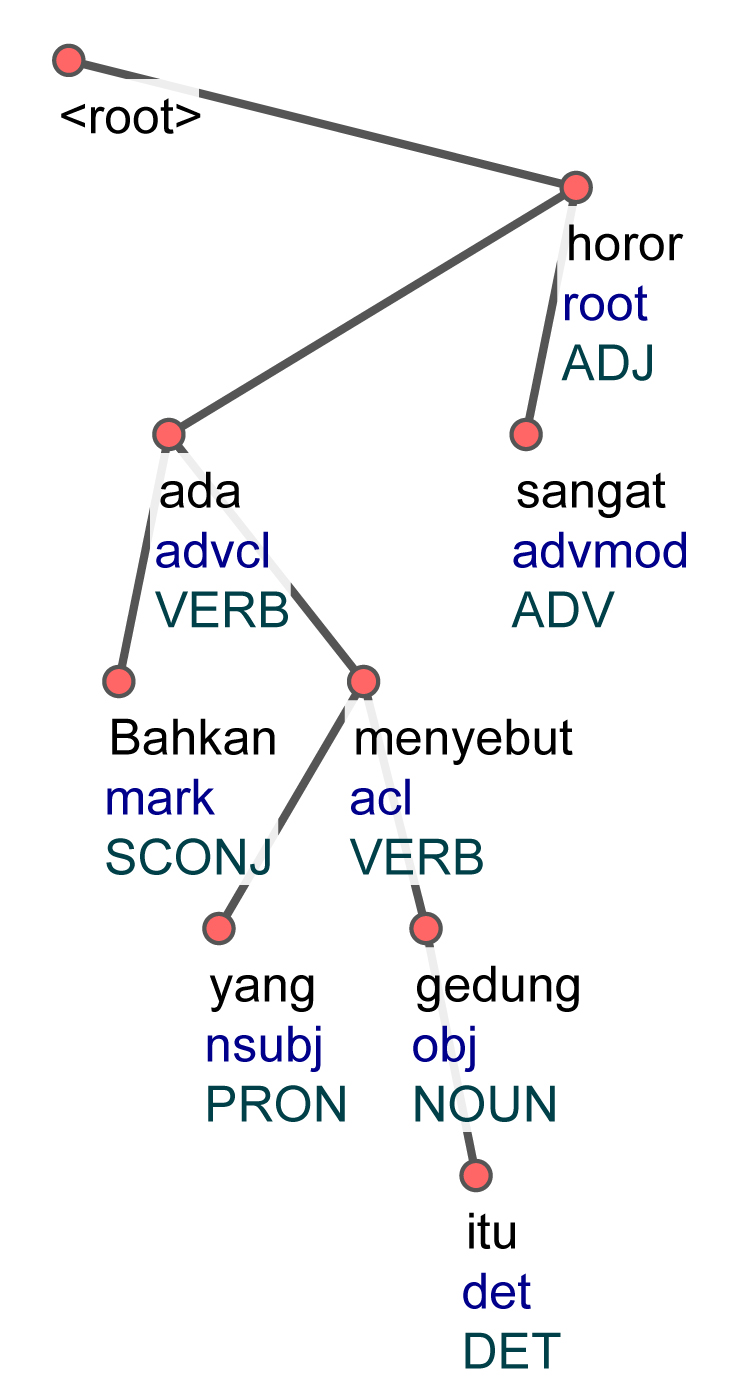
\includegraphics[width=0.8
	\textwidth] {pics/lampiran/lampirants5385.jpg} 
	\caption{lampirants5385} 
	\label{fig:lampirants5385} 
\end{figure}

\begin{figure}
	\centering 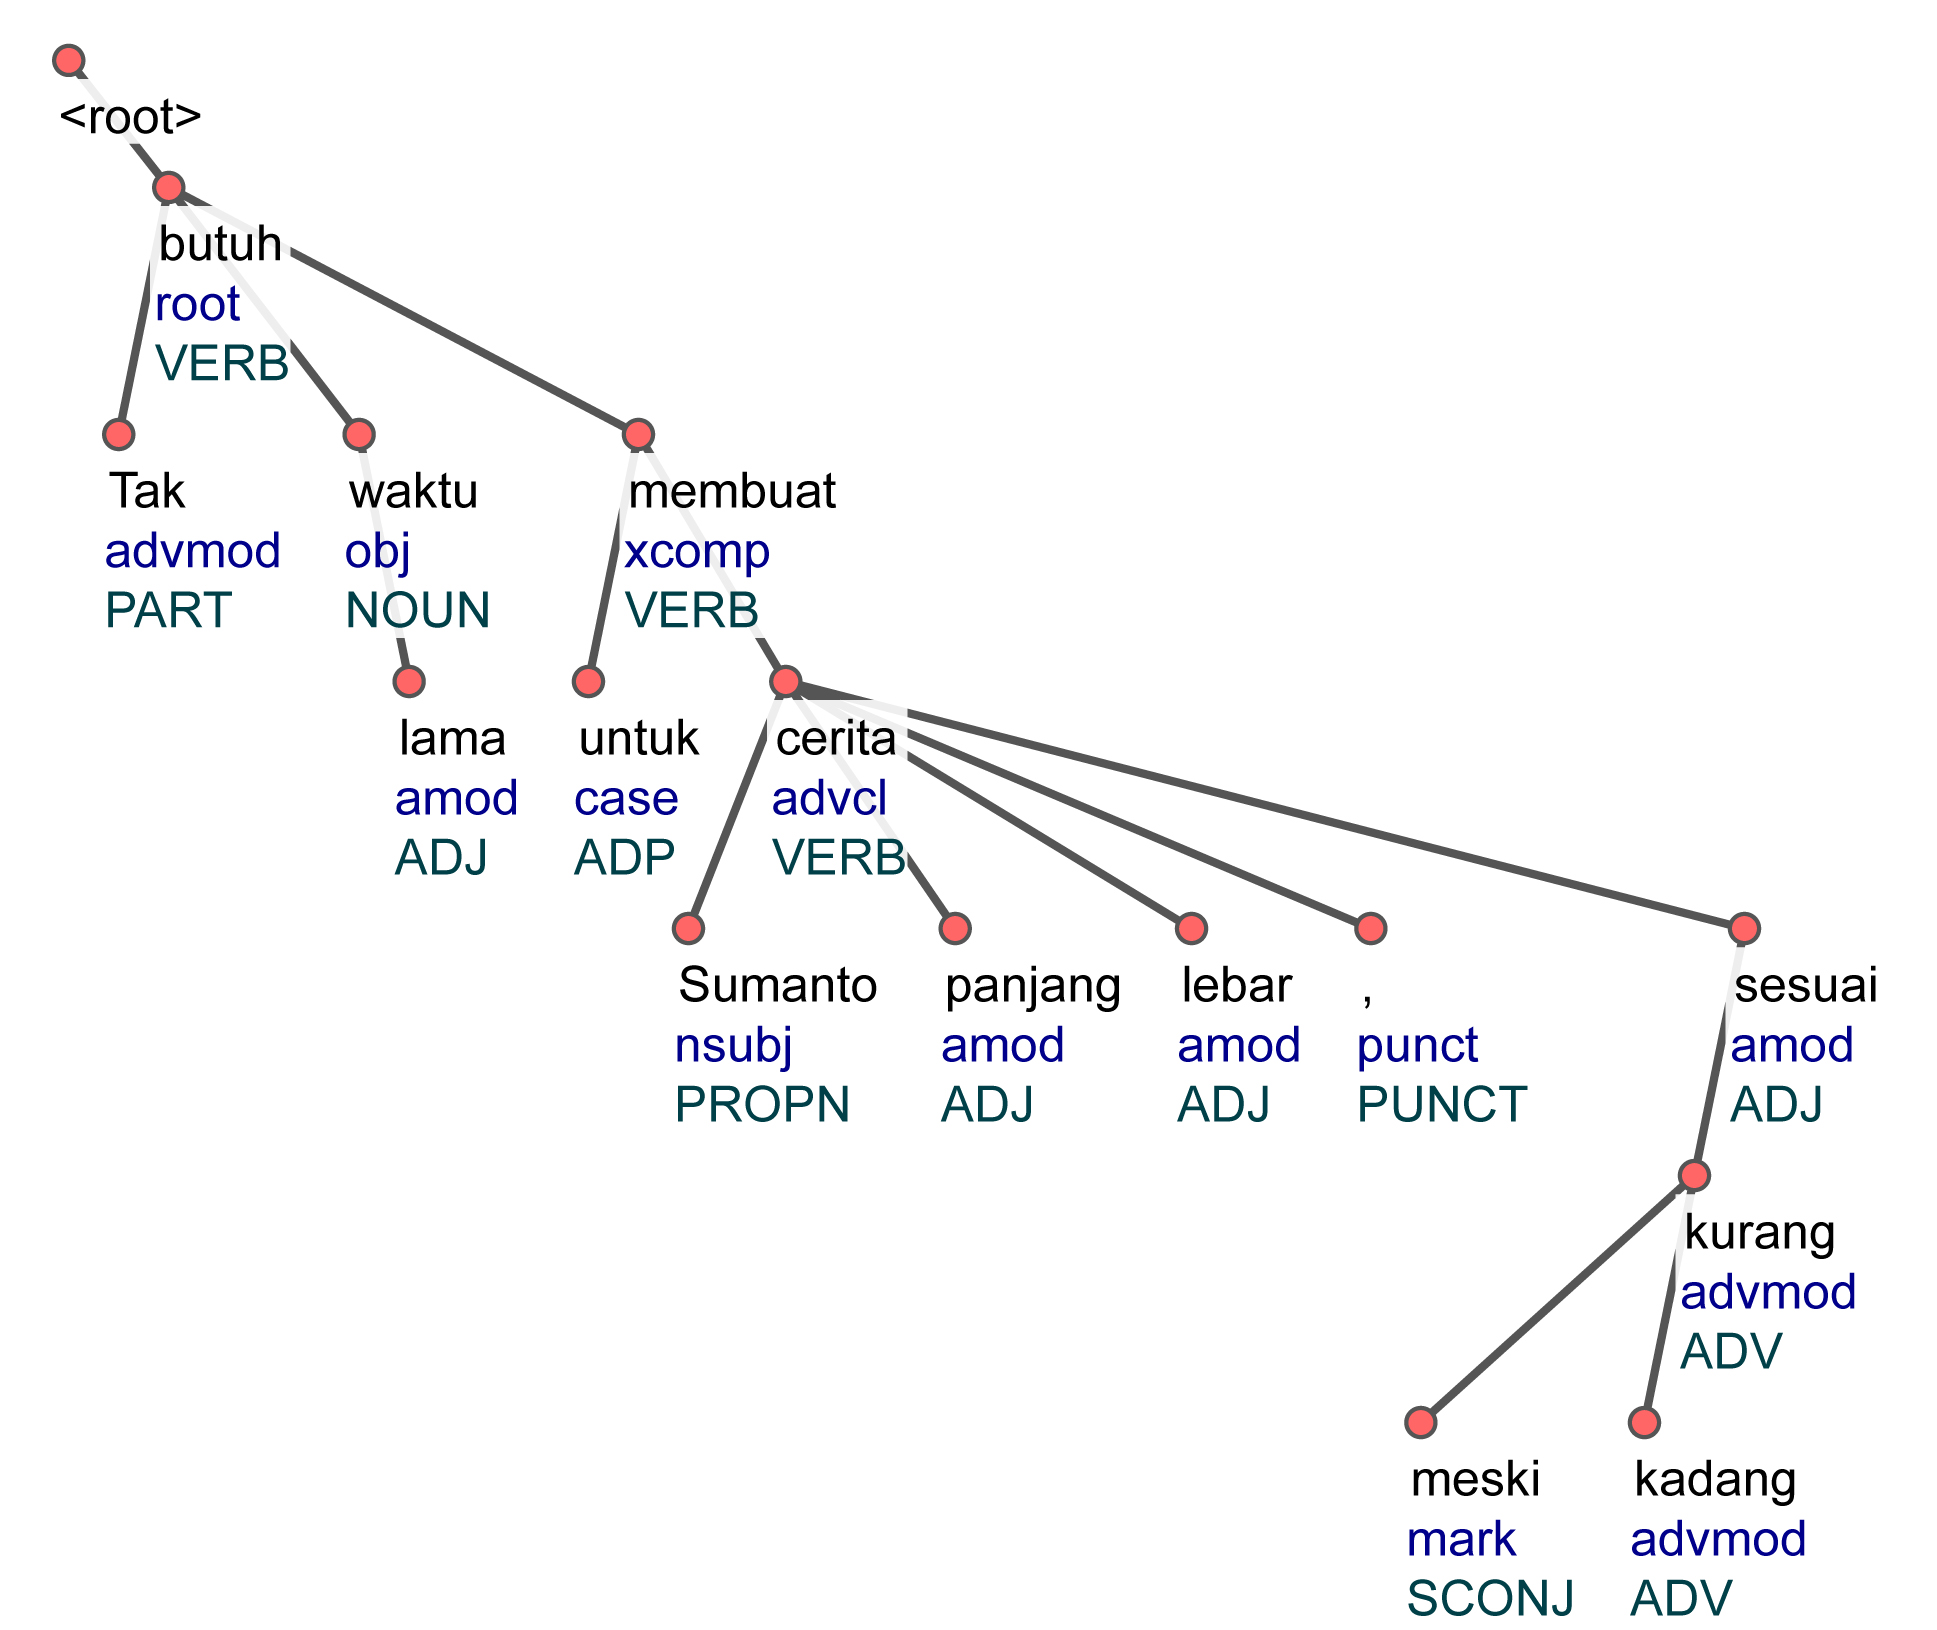
\includegraphics[width=0.8
	\textwidth] {pics/lampiran/lampirants6703.jpg} 
	\caption{lampirants6703} 
	\label{fig:lampirants6703} 
\end{figure}

\begin{figure}
	\centering 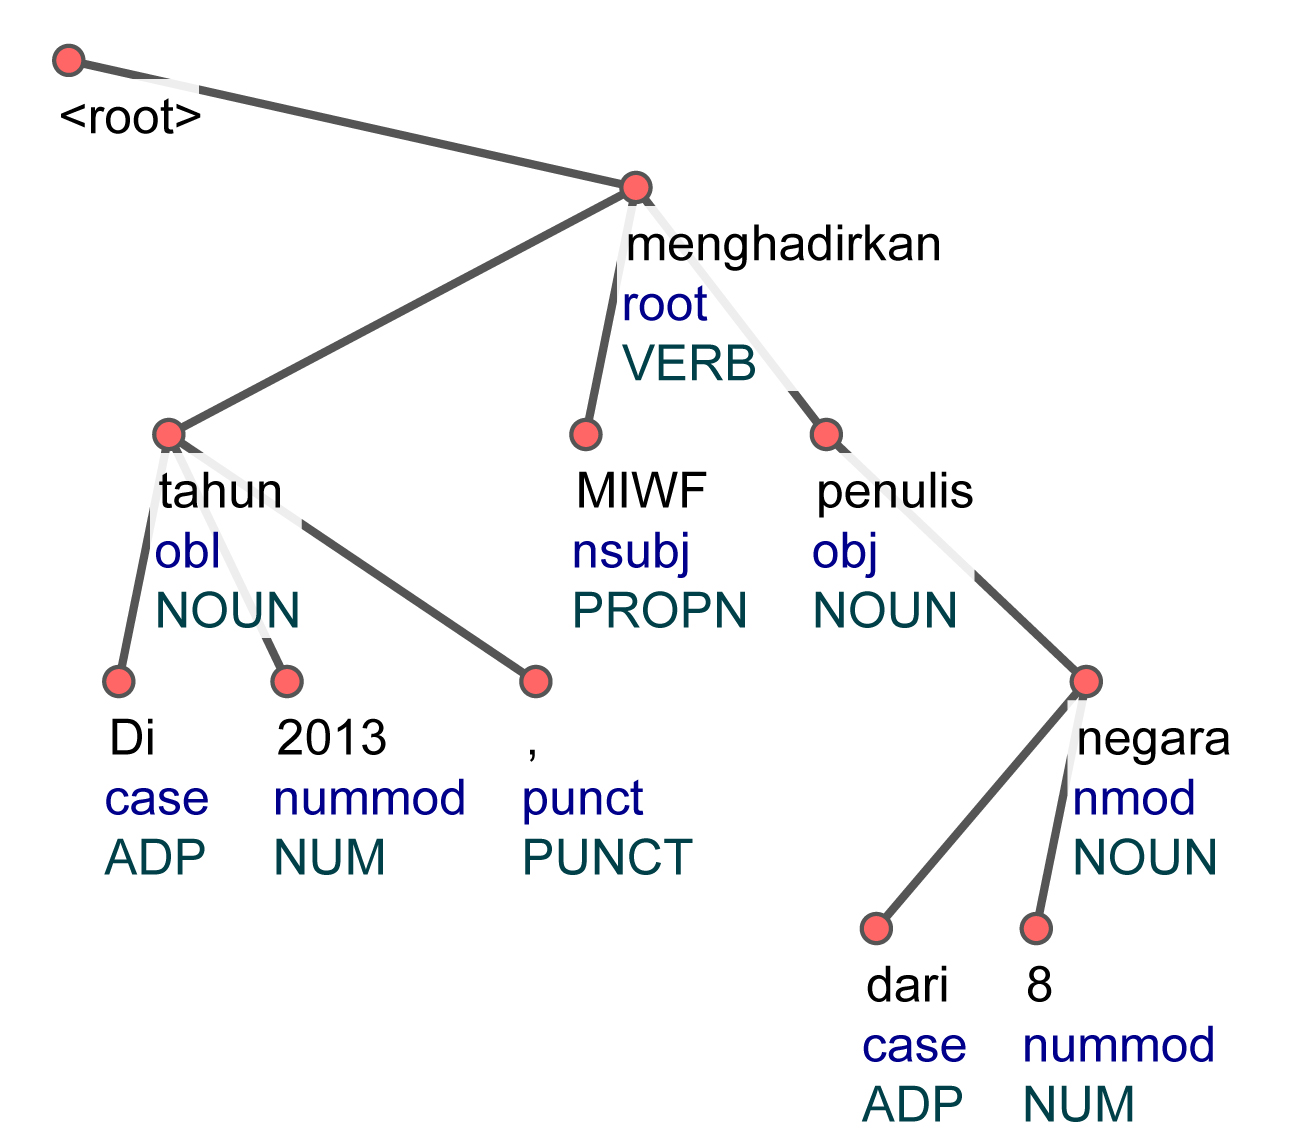
\includegraphics[width=0.8
	\textwidth] {pics/lampiran/lampirants7706.jpg} 
	\caption{lampirants7706} 
	\label{fig:lampirants7706} 
\end{figure}

%%

\begin{figure}
	\centering 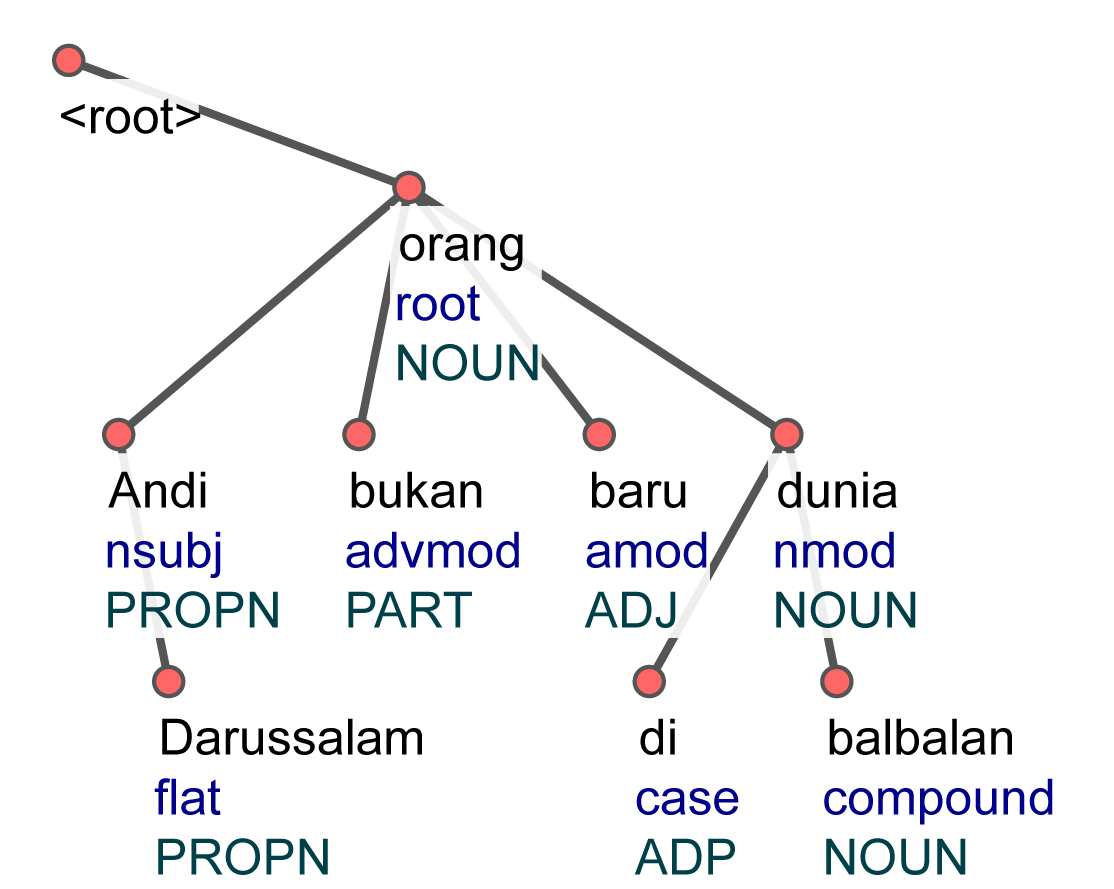
\includegraphics[width=0.8
	\textwidth] {pics/lampiran/lampirants8990.jpg} 
	\caption{lampirants8990} 
	\label{fig:lampirants8990} 
\end{figure}

\begin{figure}
	\centering 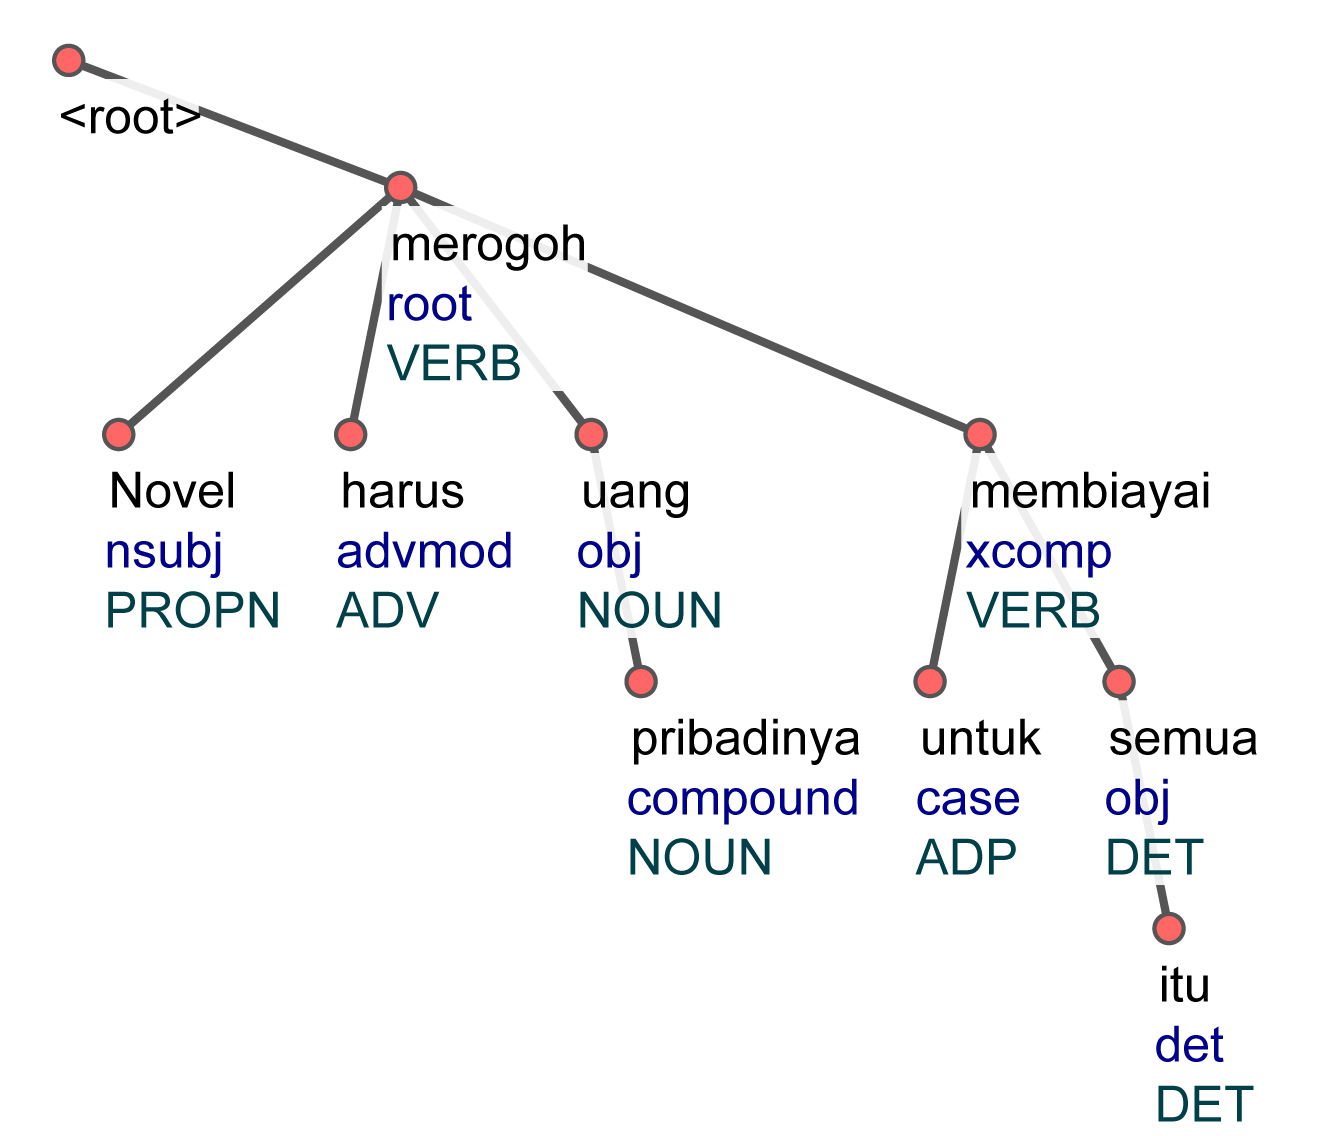
\includegraphics[width=0.8
	\textwidth] {pics/lampiran/lampirants9184.jpg} 
	\caption{lampirants9184} 
	\label{fig:lampirants9184} 
\end{figure}
